\documentclass[11pt]{beamer}
\usetheme{PaloAlto}
\usecolortheme{spruce}
\usepackage[spanish]{babel}
\usefonttheme{professionalfonts}
\usefonttheme{serif}
\usepackage{minted}
\usepackage{fontspec}
\setmainfont{Liberation Serif}
\usepackage{amsmath}
\usepackage{amsfonts}
\usepackage{amssymb}
\usepackage{graphicx}
\usepackage{menukeys} 
%Se configura minted
\definecolor{bg}{rgb}{0.95,0.95,0.95}
%\newminted{python}{fontsize=\scriptsize, 
%		   linenos,
%		   numbersep=8pt,
%		   gobble=4,
%		   frame=lines,
%		   bgcolor=bg,
%		   framesep=3mm} 
%\newminted{pycon}{bgcolor=bg, linenos=true, tabsize=4}
%\newcommand{\tab}[1][1cm]{\hspace*{#1}}

\author{Nelson David Pérez Garecía\\}
\title{Introducción a SEISAN:\\Sesión I}
%\setbeamercovered{transparent} 
%\setbeamertemplate{navigation symbols}{} 
%\logo{} 
\institute{Red Sismológica Nacional, \\Servicio Geológico Colombiano} 
\date{} 
%\subject{} 
\begin{document}

\begin{frame}
\titlepage
\begin{center}
\begin{figure}

\includegraphics[scale=0.15]{Logo-SGC.jpg}
\end{figure}
\end{center}
\end{frame}

\begin{frame}
\tableofcontents
\end{frame}

\section{Introducción}
\subsection{Prerrequisitos}
\begin{frame}{Prerrequisitos}
Para el uso de SEISAN es aconsejable tener conocimiento mínimo en los siguientes temas:
\begin{itemize}
\item Sismología de terremotos.
\pause
\item Sitema operativo UNIX/LINUX. 
\end{itemize}
\end{frame}

\begin{frame}{Prerrequisitos (Linux)}
Algunos comandos básicos de Linux:
\begin{table}
{\small
\begin{tabular}{|c|c|c|}
\hline 
 {\bf Comando} & {\bf Descripción} & {\bf Ejemplos}\\ 
\hline 
cat  & Concatena y muestra un archivo & cat /etc/passwd\\ 
\hline 
ls & Lista los archivos del directorio & ls /bd/seismo \\ 
\hline 
cd & Cambia el directorio & cd /tmp \\ 
\hline 
cp & Copia archivos & cp foo foo.backup \\ 
\hline 
mkdir & Crea un directorio & mkdir seismo \\ 
\hline 
mv & Mueve un archivo a un directorio & mv a.out prog1 \\ 
\hline 
more/less & Visualiza página a página un archivo & more foo.txt \\ 
\hline 
rm  & Borra un archivo & rm foo.c \\ 
\hline 
rm -r  & Borra un directorio & rm -r /bd/seismo\\ 
\hline 
pwd & Muestra la ruta del directorio actual & pwd \\ 
\hline
ssh & Conección a un servidor remoto & ssh -X seismo@...\\
\hline
\end{tabular}}
\end{table} 
\end{frame}

\begin{frame}
Ingresemos a la terminal ...\\

\begin{figure}

\includegraphics[scale=0.5]{terminal.png}
\end{figure}
\end{frame}

\subsection{¿Qué es SEISAN?}
\begin{frame}{¿Qué es SEISAN?}
\begin{figure}
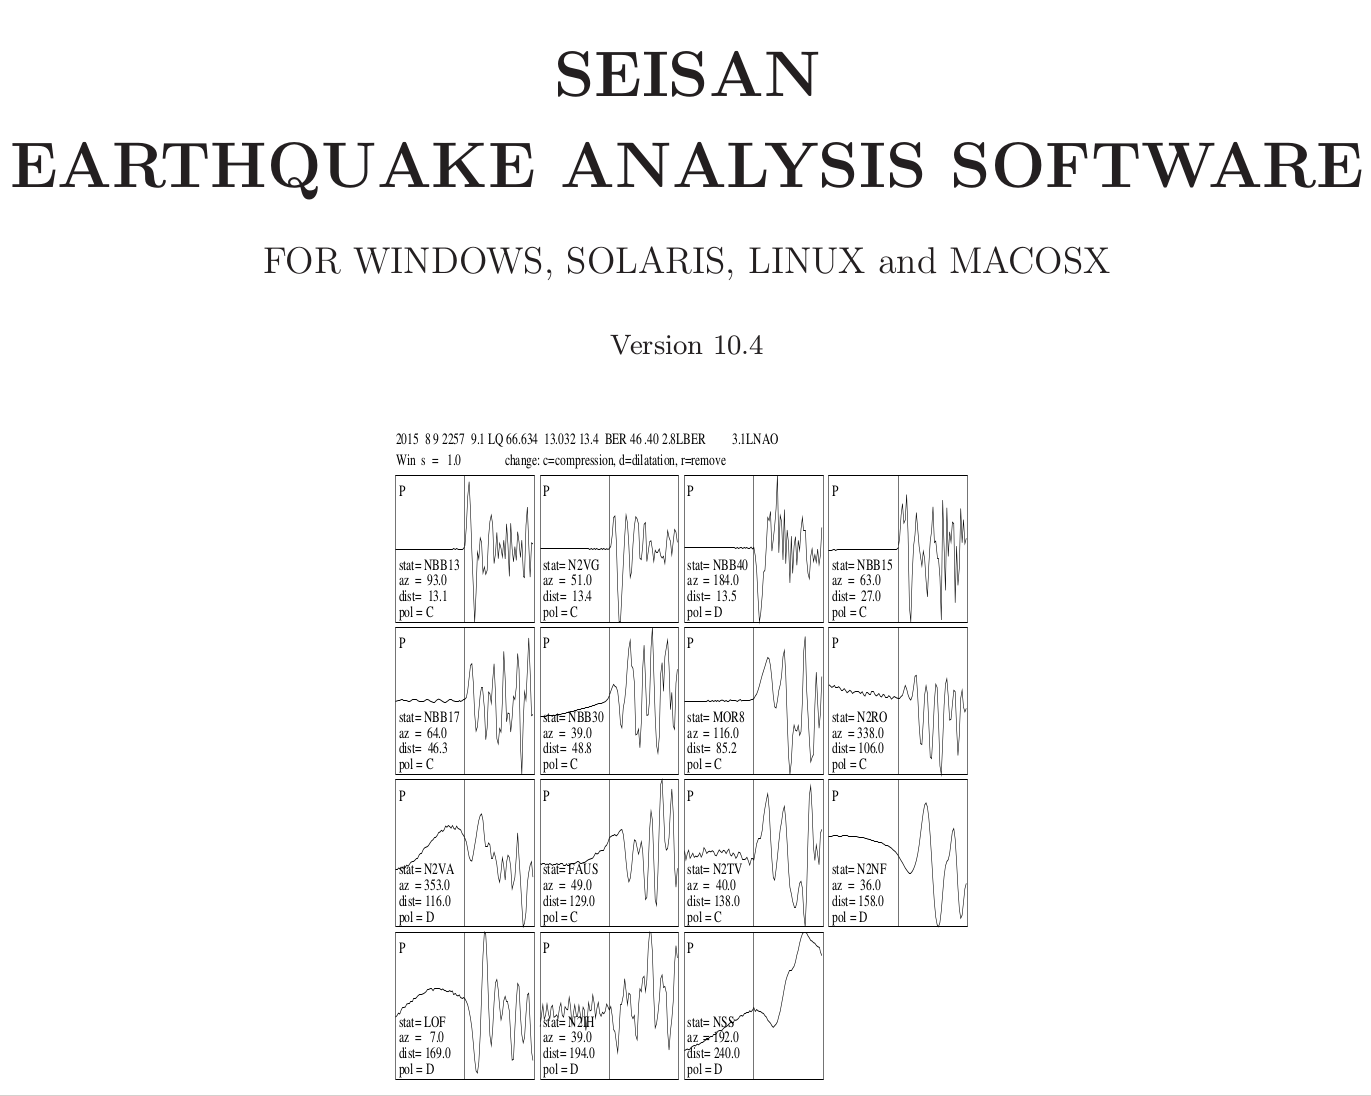
\includegraphics[scale=0.2]{seisan_portada.png}
\end{figure}
\end{frame}
\begin{frame}{SEISAN}
SEISAN (SEISmic ANalysis System) esta constituido por una base de datos de eventos sísmicos y un conjunto de programas que permiten analizar de forma rutinaria los eventos que ocurren tanto local como globalmente. 
\begin{itemize}
\item Permite almacenar y consultar los eventos sísmicos en un formato estándar.\\
\pause
\item Permite el procesamiento de catálogos extensos de eventos sísmicos.\\
\pause
\item Procesamiento básico (rutina) y avanzado en sismología.
\pause
\item Es un software multiplataforma (Linux, MacOS, Windows).\\
\pause
\end{itemize}
\end{frame}
\begin{frame}{SEISAN}
Donde se encuentrar SEISAN
\begin{itemize}
\item \url{http://seisan.info/}
\item \url{https://www.youtube.com/watch?v=KJH3ktGL_K0}
\item Localmente en {\tt /bd/seismo/INF/}
\end{itemize}
\end{frame}

\section{Estructura de SEISAN}
\subsection{Estructura básica}
\begin{frame}{Estructura de SEISAN}
\begin{figure}
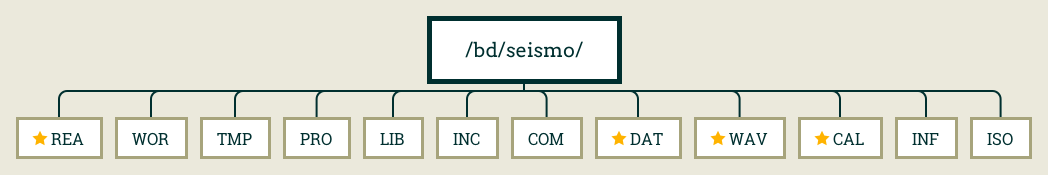
\includegraphics[scale=0.28]{estructura_seisan_1.png}
\end{figure}
\end{frame}

\begin{frame}{Estructura de SEISAN}
\begin{figure}
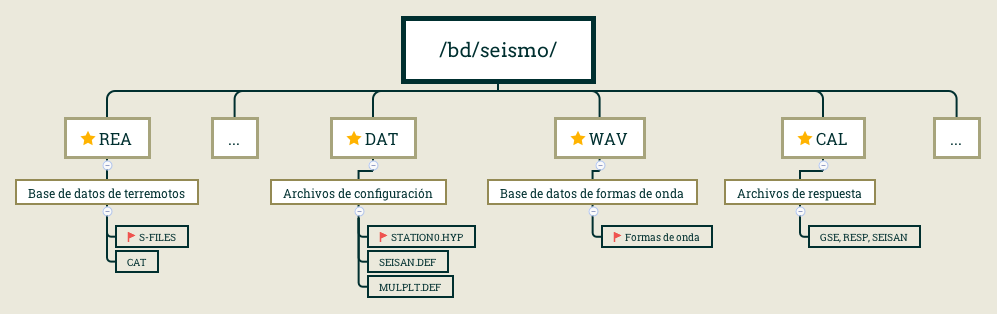
\includegraphics[scale=0.28]{estructura_seisan2.png}
\end{figure}
\end{frame}

\begin{frame}{Estructura de SEISAN}
\begin{figure}
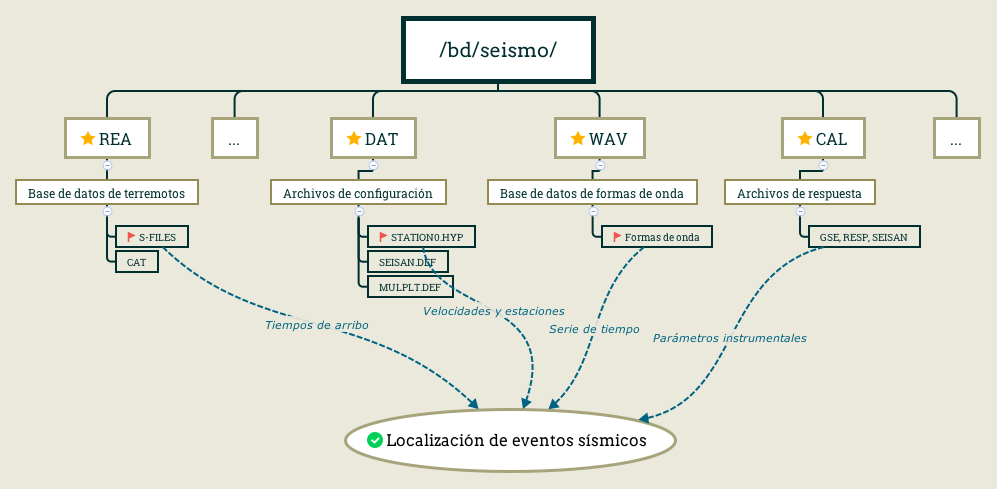
\includegraphics[scale=0.28]{estructura_seisan3.png}
\end{figure}
\end{frame}

\subsection{WAV}
\begin{frame}{WAV}
WAV es la base de datos de formas de onda. Las formas de onda son series de tiempo de los registros de la velocidad del suelo. Estas formas de onda se almacenan en formato digital para facilitar su intercambio y procesamiento.\\

\begin{figure}
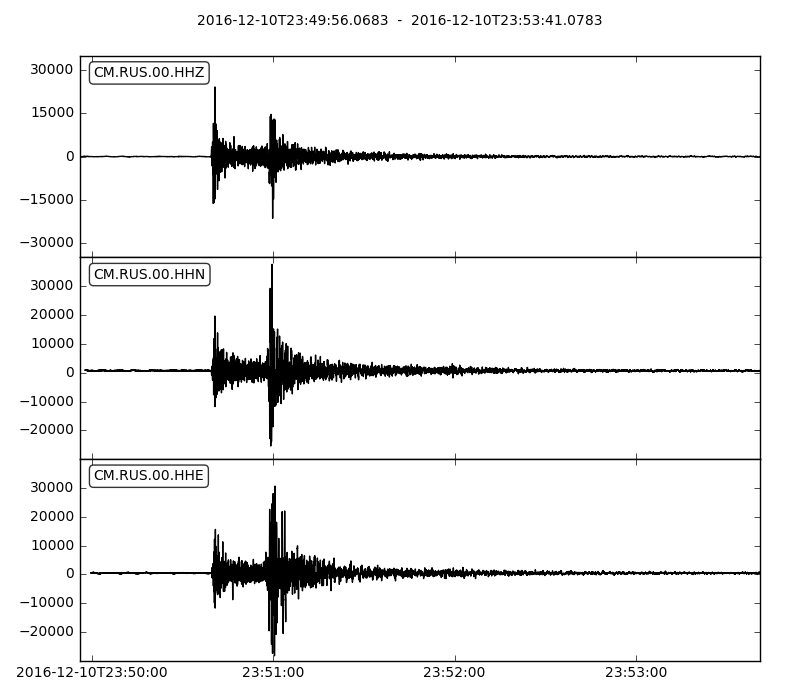
\includegraphics[scale=0.2]{sismo_RUS.png}
\caption{Sismograma digital de un evento sísmico.}
\end{figure}
\end{frame}

\begin{frame}{Formatos de sismogramas digitales}
Existen diferentes formatos para almacenar formas de onda:
\begin{itemize}
\item Formato SEISAN.\\
\pause
\item Formato SAC (Seismic Analysis Code).\\
\pause
\item Passcal.\\
\pause
\item GCF (Guralp Compressed Format).\\
\pause
\item Standard for the Exchange of Earthquake Data (SEED).\\
\pause 
\end{itemize}
Estos formatos almacenan la información en canales simples y volúmenes multicanal junto con los metadatos de cada serie de tiempo. 
\end{frame}

\begin{frame}
Los metadatos básicos de una serie de tiempo en formato miniSEED son:
\begin{center}
{\tt       network: CM\\
         station: RUS\\
        location: 00\\
         channel: HHZ\\
       starttime: 2009-08-24T00:20:03.000000Z\\
         endtime: 2009-08-24T00:20:32.990000Z\\
   sampling\_rate: 100.0\\
              delta: 0.01\\
            npts: 3000\\}
\end{center}
\end{frame}


\subsubsection{Comando {\tt mulplt}}
\begin{frame}{WAV: comando {\tt mulplt}}
Este es el comando que permite la visualización de formas de onda en SEISAN.
\begin{figure}
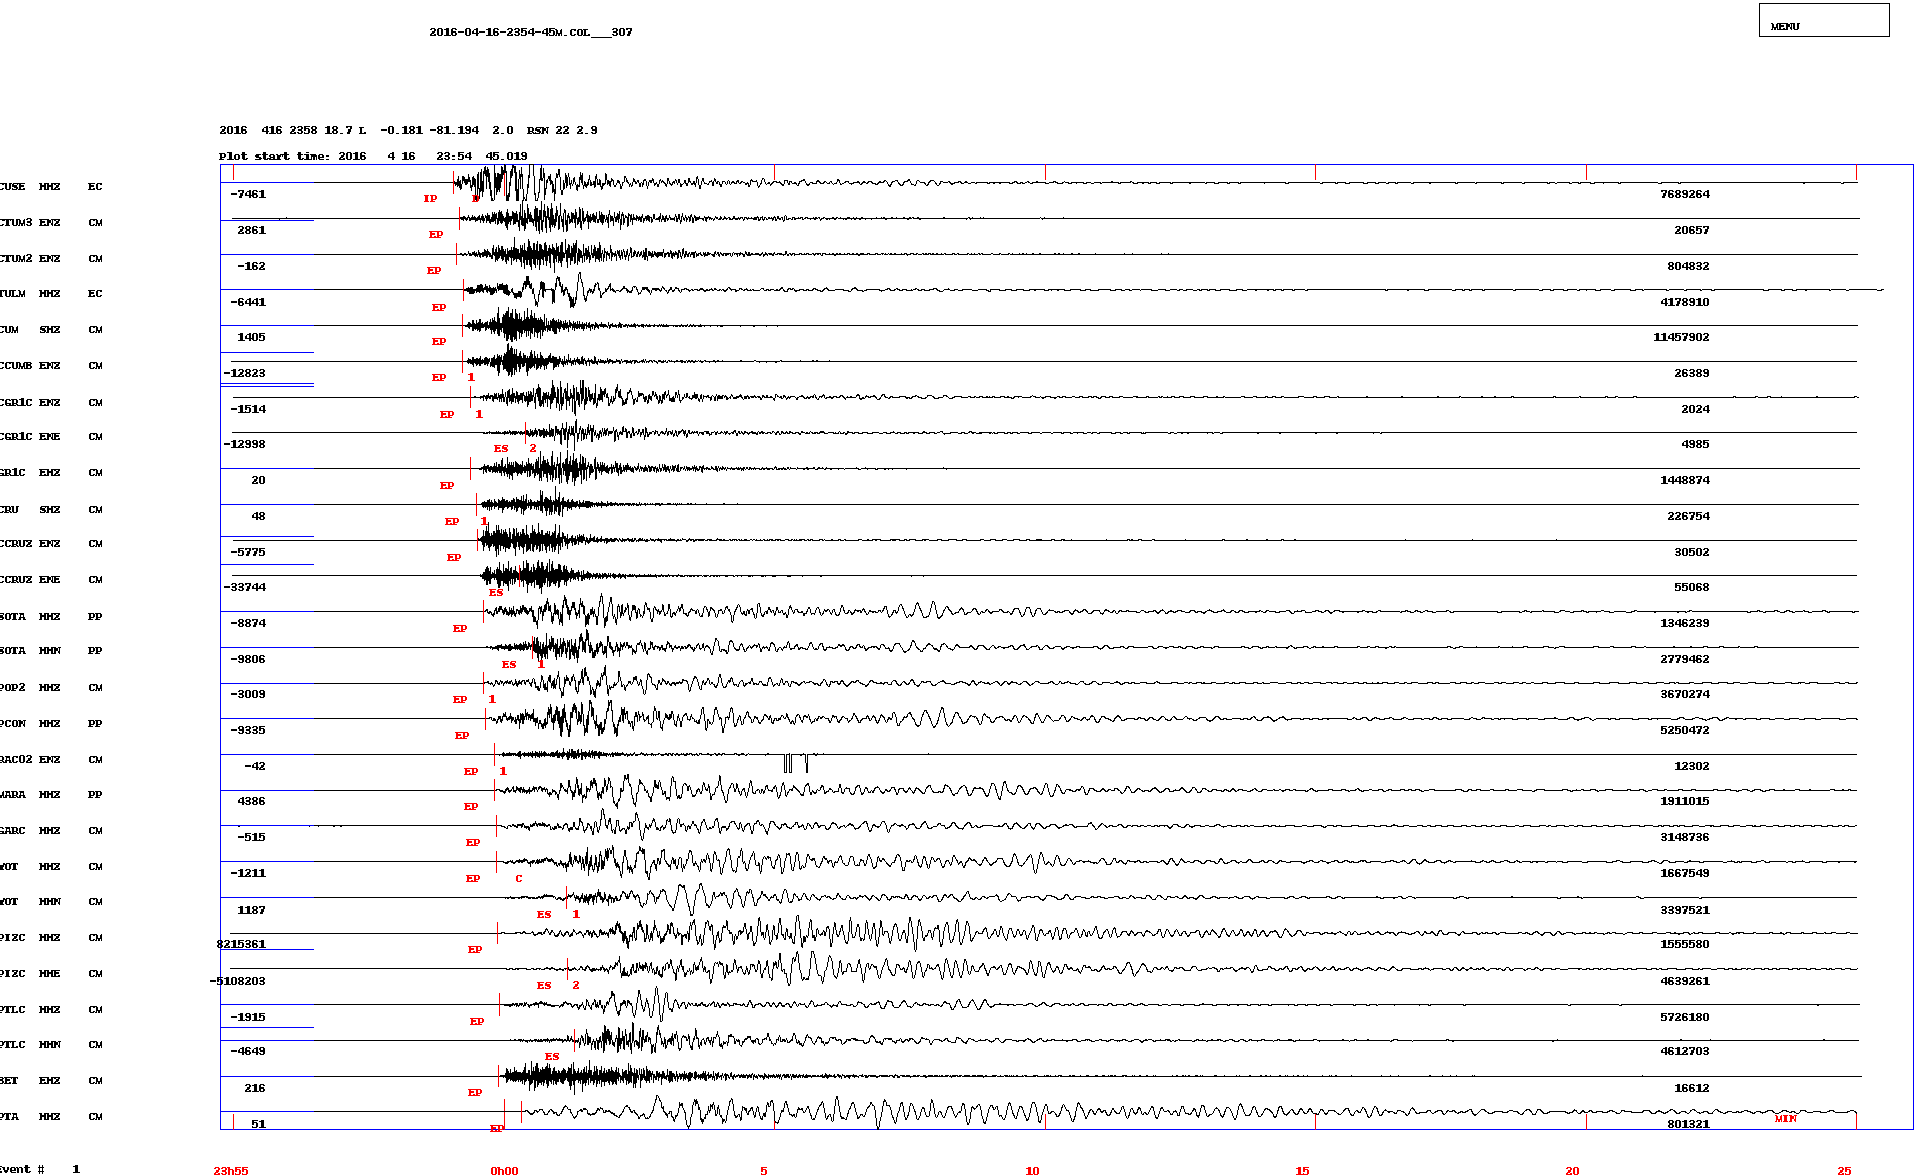
\includegraphics[scale=0.13]{traza.png}
\end{figure}

Las archivos de formas de onda tienen nombres como {\tt 2014-06-25-0726-38M.COL\_\_\_256}.
\end{frame}

\begin{frame}{WAV: comando {\tt mulplt}}
Al iniciar {\tt mulplt} desde la terminal se observa el siguiente menú:\\
{\tt 
Filename, number, filenr.lis (all)\\
  Continuous SEISAN data base: cont\\ 
  Large SEED volume: conts\\
  Archive: arc\\
  Make a choice\\
} 

El comando no admite volúmenes de duración mayor a 2 horas directamente. Para esto se utiliza la opción {\tt conts}.
\end{frame}

\begin{frame}{Opciones en {\tt mulplt}}
El comando {\tt mulplt} tiene diferentes opciones interactivas que se pueden observar como botones desde la parte superior de las ventanas
%\begin{figure}
%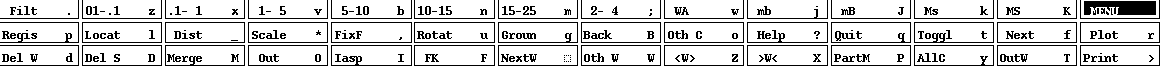
\includegraphics[scale=0.3]{menu.png}
%\end{figure}
\begin{table} 
\begin{tabular}{|c|c|}
\hline 
{\bf Comando} & {\bf Descripción} \\ 
\hline 
{\tt q} & Salir de {\tt mulplt} \\ 
\hline 
\keys{\tab} & Cambiar páginas de canales \\ 
\hline 
{\tt f} & Pasar a la siguiente forma de onda  \\ 
\hline 
{\tt B} & Forma de onda anterior \\ 
\hline 
{\tt o} & Muestra menú de canales\\ 
\hline 
{\tt r} & refresca la vista de multicanales \\ 
\hline
{\tt t} & vista de canal individual \\ 
\hline 
\end{tabular}
\end{table}
{\scriptsize Nota: estas opciones funcionan en el teclado americano ({\tt US})}
\end{frame}

\begin{frame}{Opciones en {\tt mulplt}}
\begin{table}
\begin{tabular}{|c|c|}
\hline
{\bf Comando} & {\bf Descripción}\\ 
\hline
{\tt p} & Registrar evento sísmico nuevo \\ 
\hline 
Cursor sobre señal + {\tt 1} & Marca fase IP  \\ 
\hline 
Cursor sobre señal + {\tt 2} & Marca fase EP \\ 
\hline 
Cursor sobre señal + {\tt 8} & Marca fase ES \\ 
\hline 
{\tt w} + selección de ventana & Filtro Wood-Anderson \\ 
\hline
Cursor sobre señal + {\tt a} & Marca amplitud pico a pico\\
\hline 
\keys{\shift} + {\tt A} & Marca amplitud automática \\ 
\hline 
{\tt l} & Localiza con Hypocenter \\ 
\hline 
{\tt op} & Selecciona caanles con fases picadas \\ 
\hline 
\end{tabular}
\end{table}
{\scriptsize Nota: estas opciones funcionan en el teclado americano ({\tt US})} 
\end{frame}

\begin{frame}{Opciones en {\tt mulplt}}
Filtros:\\
\begin{table}
\begin{tabular}{|c|c|}
\hline
{\bf Comando} & {\bf Filtro} \\
\hline
{\tt v + r} & Pasabanda 1 - 5 Hz \\ 
\hline 
{\tt b + r} & Pasabanda 5 - 10 Hz \\ 
\hline 
{\tt x + r} & Pasabanda 0.1 - 1.0 Hz \\ 
\hline 
{\tt b + r} & Pasabanda 0.01 - 1 Hz \\ 
\hline 
{\tt n + r} & Pasabanda 10 - 15 Hz \\  
\hline 
{\tt Punto + $f_{min}$ - $f_{max}$} & Pasabanda $f_{min}$ - $f_{max}$ Hz \\  
\hline
{\tt ; + r} & Pasabanda 2 - 4 Hz \\  
\hline
Coma $\rightarrow$ Filtro & Mantiene filtro \\  
\hline
\end{tabular} 
\end{table}
{\scriptsize Nota: estas opciones funcionan en el teclado americano ({\tt US})}
\end{frame}

\begin{frame}{Opciones en {\tt mulplt}}
Pesos:\\
\begin{table}
\begin{tabular}{|c|c|c|}
\hline 
 {\bf Comando} & {\bf Peso} & {\bf valor} \\ 
\hline 
\keys{\shift} + 1 & 1 & 75 \% de certeza  \\ 
\hline 
\keys{\shift} + 2 & 2 & 50 \% de certeza \\ 
\hline 
\keys{\shift} + 3 & 3 & 25 \% de certeza \\ 
\hline 
\keys{\shift} + 4 & 4 & 100 \% de incertidumbre \\ 
\hline
\keys{\shift} + 9 & 9 & Utiliza tiempo S-P \\ 
\hline  
\end{tabular} 
\end{table}
{\scriptsize Nota: estas opciones funcionan en el teclado americano ({\tt US})}
\end{frame}


\begin{frame}{WAV: comando {\tt dirf}}
El comando {\tt dirf} crea una lista numerada de archivos:\\
{\small \tt 
 \$ dirf *.COL*\\
 \#  1  2014-06-25-0726-38M.COL\_\_\_ 256 \\                                        
 \#  2  2016-09-25-0500-00M.COL\_\_\_ 327 \\                                        
 \#  3  2016-09-26-1633-25M.COL\_\_\_ 336 \\
}
\end{frame}



\subsection{REA}
\begin{frame}[fragile]{REA}
Es la base de datos de soluciones de hipocentros de eventos sísmicos. Para ingresar:\\
\begin{minted}{bash}
$cd /bd/seismo/REA
\end{minted}
\begin{minted}{bash}
$re
\end{minted}
\end{frame}

\begin{frame}{REA}
La base de datos REA está compuesta por archivos de texto plano conocidos cómo S-files:\\
\begin{center}
\begin{figure}
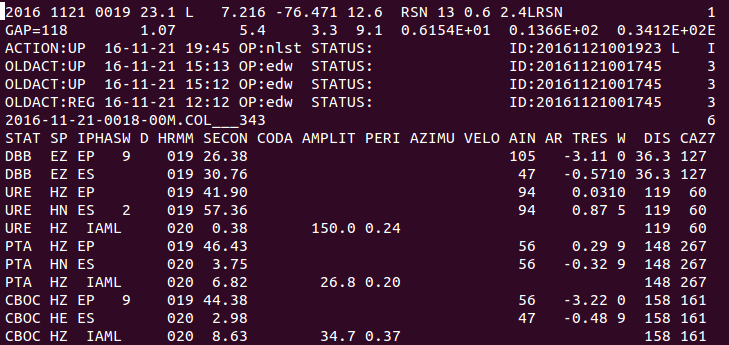
\includegraphics[scale=0.3]{sfile.png}
\end{figure}
\end{center}
El nombre típico del s-file es de la forma {\tt 21-0019-23L.S201611}.
\end{frame}
\subsubsection{Comando {\tt eev}}
\begin{frame}[fragile]{REA: comando {\tt eev}}
Con el fin de acceder a la base de datos se utiliza el comando {\tt eev}. Es un entorno que permite gestionar facilmente la base de datos de s-files.\\
{\scriptsize \tt
\$eev 20161121 BDRSN\\
2016 11 Reading events from base OPERA  3127\\ 
\# 2238 21 Nov 2016 00:19 23  L   7.216 -76.471 12.6    0.6 2.4LRSN   13  ?\\
\# 2235 21 Nov 2016 00:49 14  L   6.759 -73.132145.1    0.3 1.7LRSN    6  ?\\
}
\end{frame}

\begin{frame}{REA: comando {\tt eev}}
Los comandos básicos del entorno {\tt eev} son: 
\begin{table}
\begin{tabular}{|c|c|}
\hline 
{\bf Comando}  & {\bf Descripción} \\ 
\hline 
Ir al siguiente S-file & \keys{\return} \\ 
\hline 
Ir al S-file anterior & b \keys{\return} \\ 
\hline 
Editar evento & e \keys{\return} \\ 
\hline 
Comentar evento & com \keys{\return} \\ 
\hline
Localizar evento & l \keys{\return} \\ 
\hline
Actualizar evento & u \keys{\return} \\ 
\hline
Ver forma de onda & po \keys{\return} \\ 
\hline
Ver nombre del S-file & tt \keys{\return} \\ 
\hline
Ver nombre de forma de onda & w \keys{\return} \\ 
\hline
\end{tabular} 
\end{table}
\end{frame}

\section{Localización en SEISAN}

\begin{frame}{Localización en SEISAN}
\begin{figure}
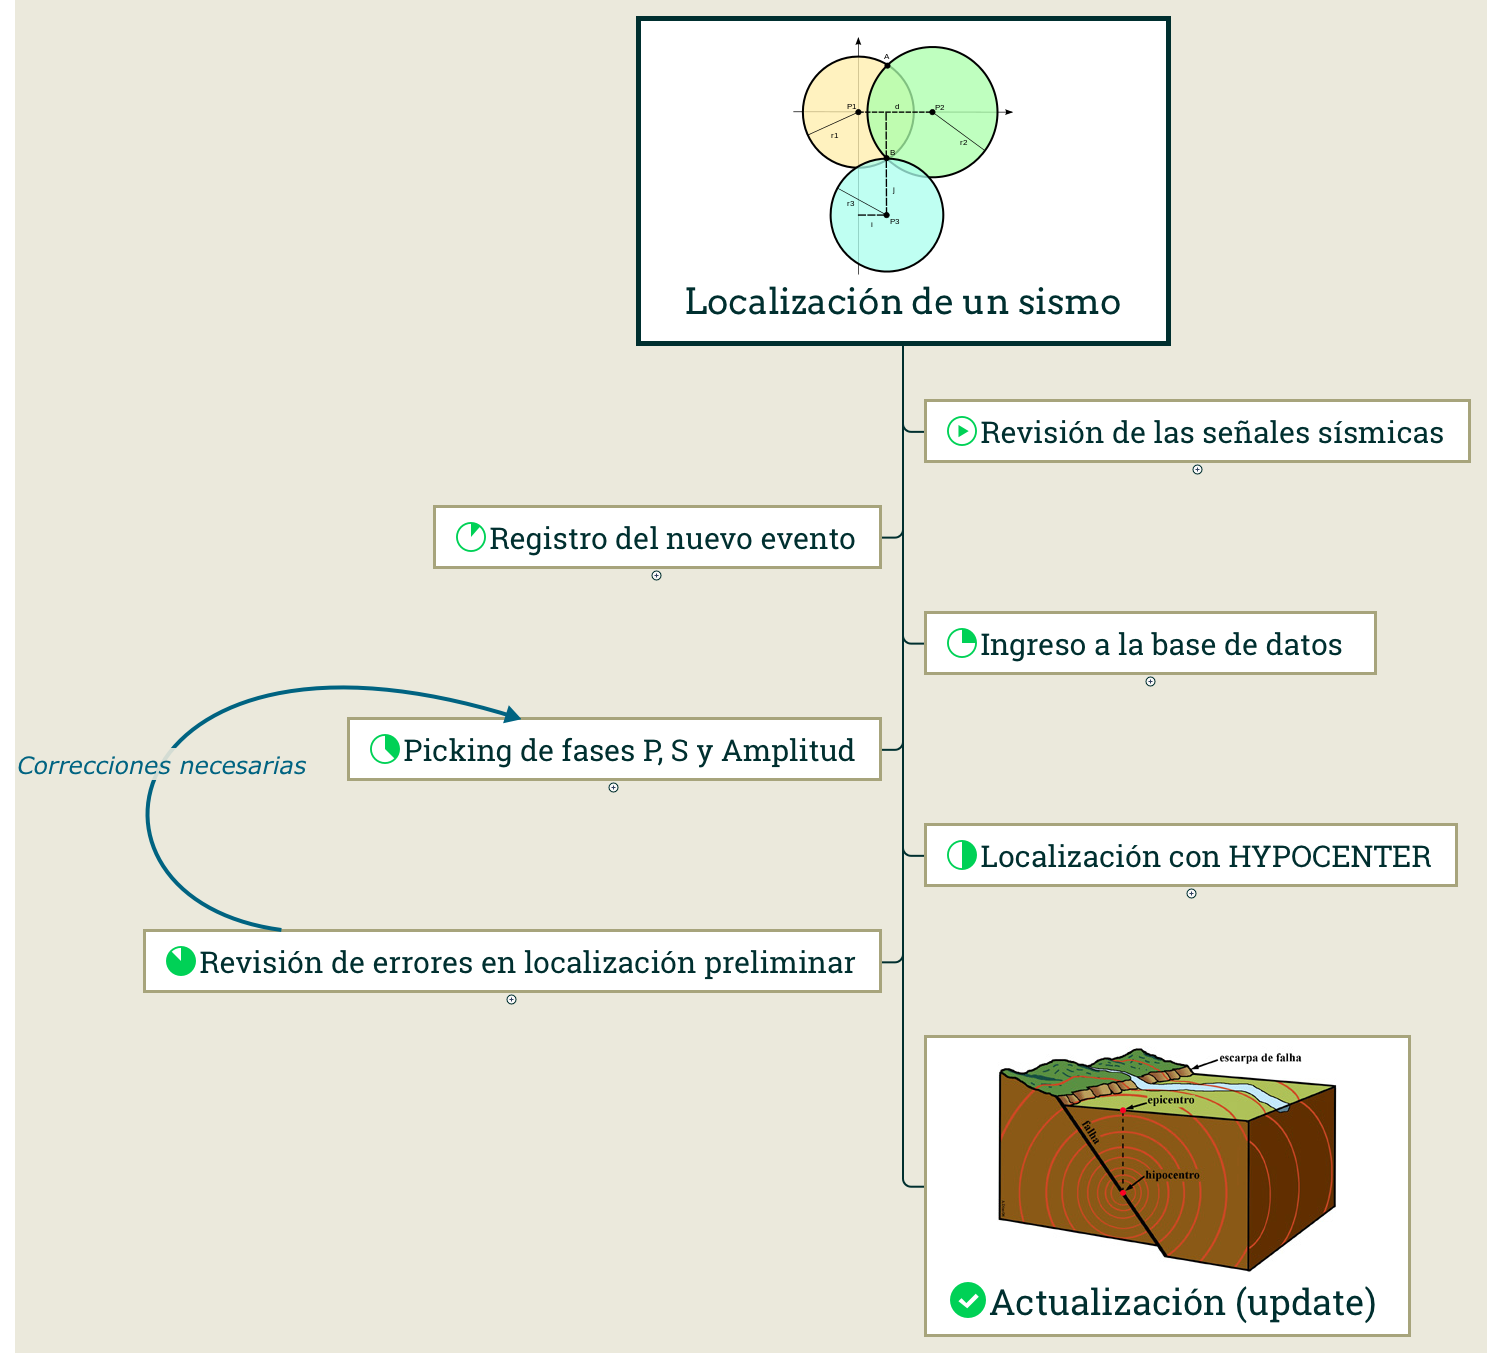
\includegraphics[scale=0.15]{localizacion_1.png}
\end{figure}
\end{frame}

\begin{frame}{Localización en SEISAN}
\begin{figure}
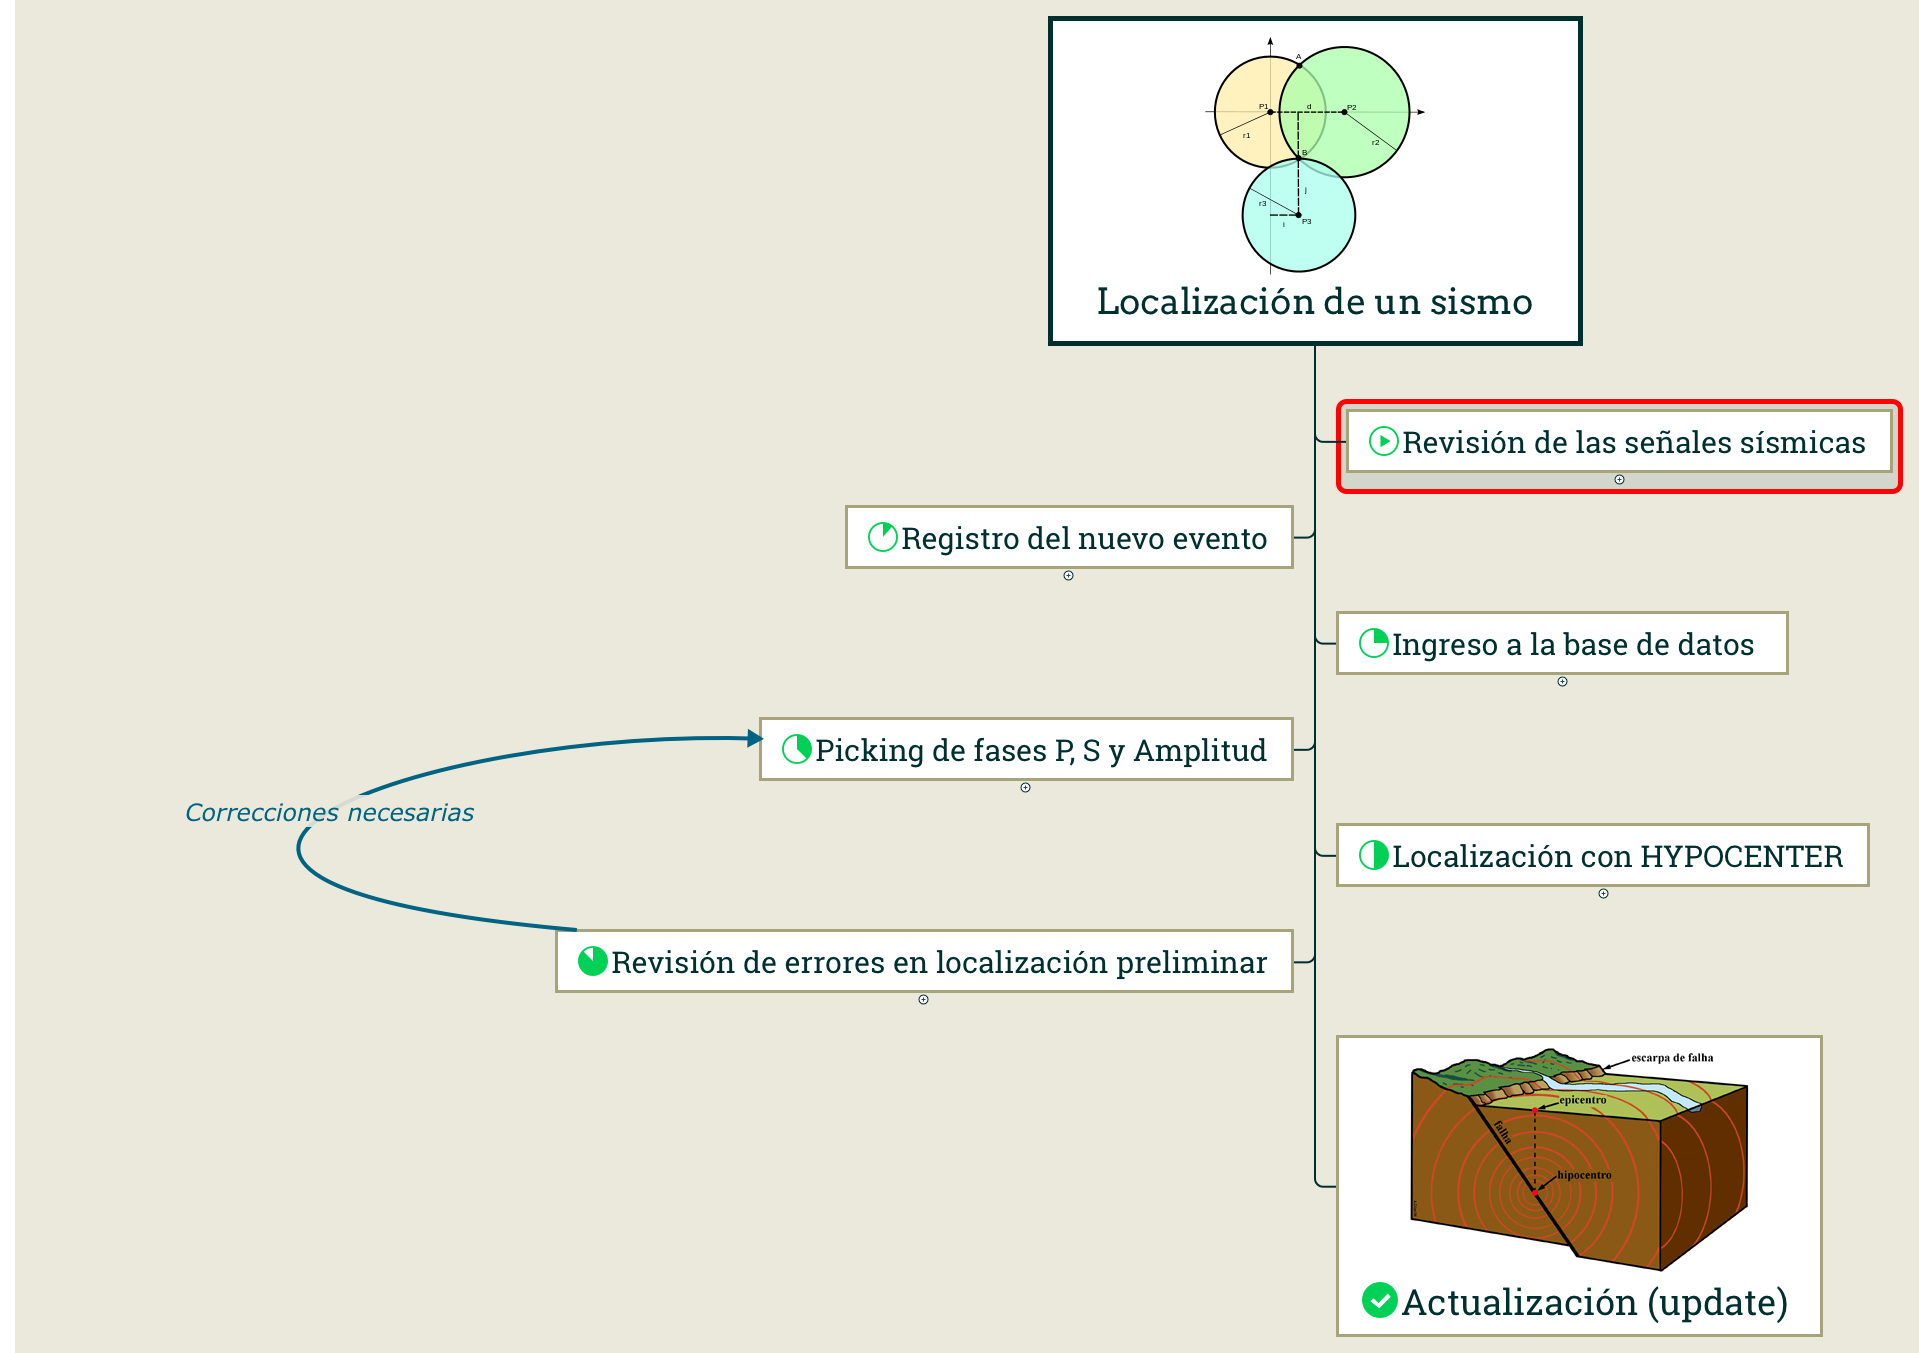
\includegraphics[scale=0.15]{localizacion_1_1.png}
\end{figure}
\end{frame}

\begin{frame}{Localización en SEISAN}
\begin{figure}
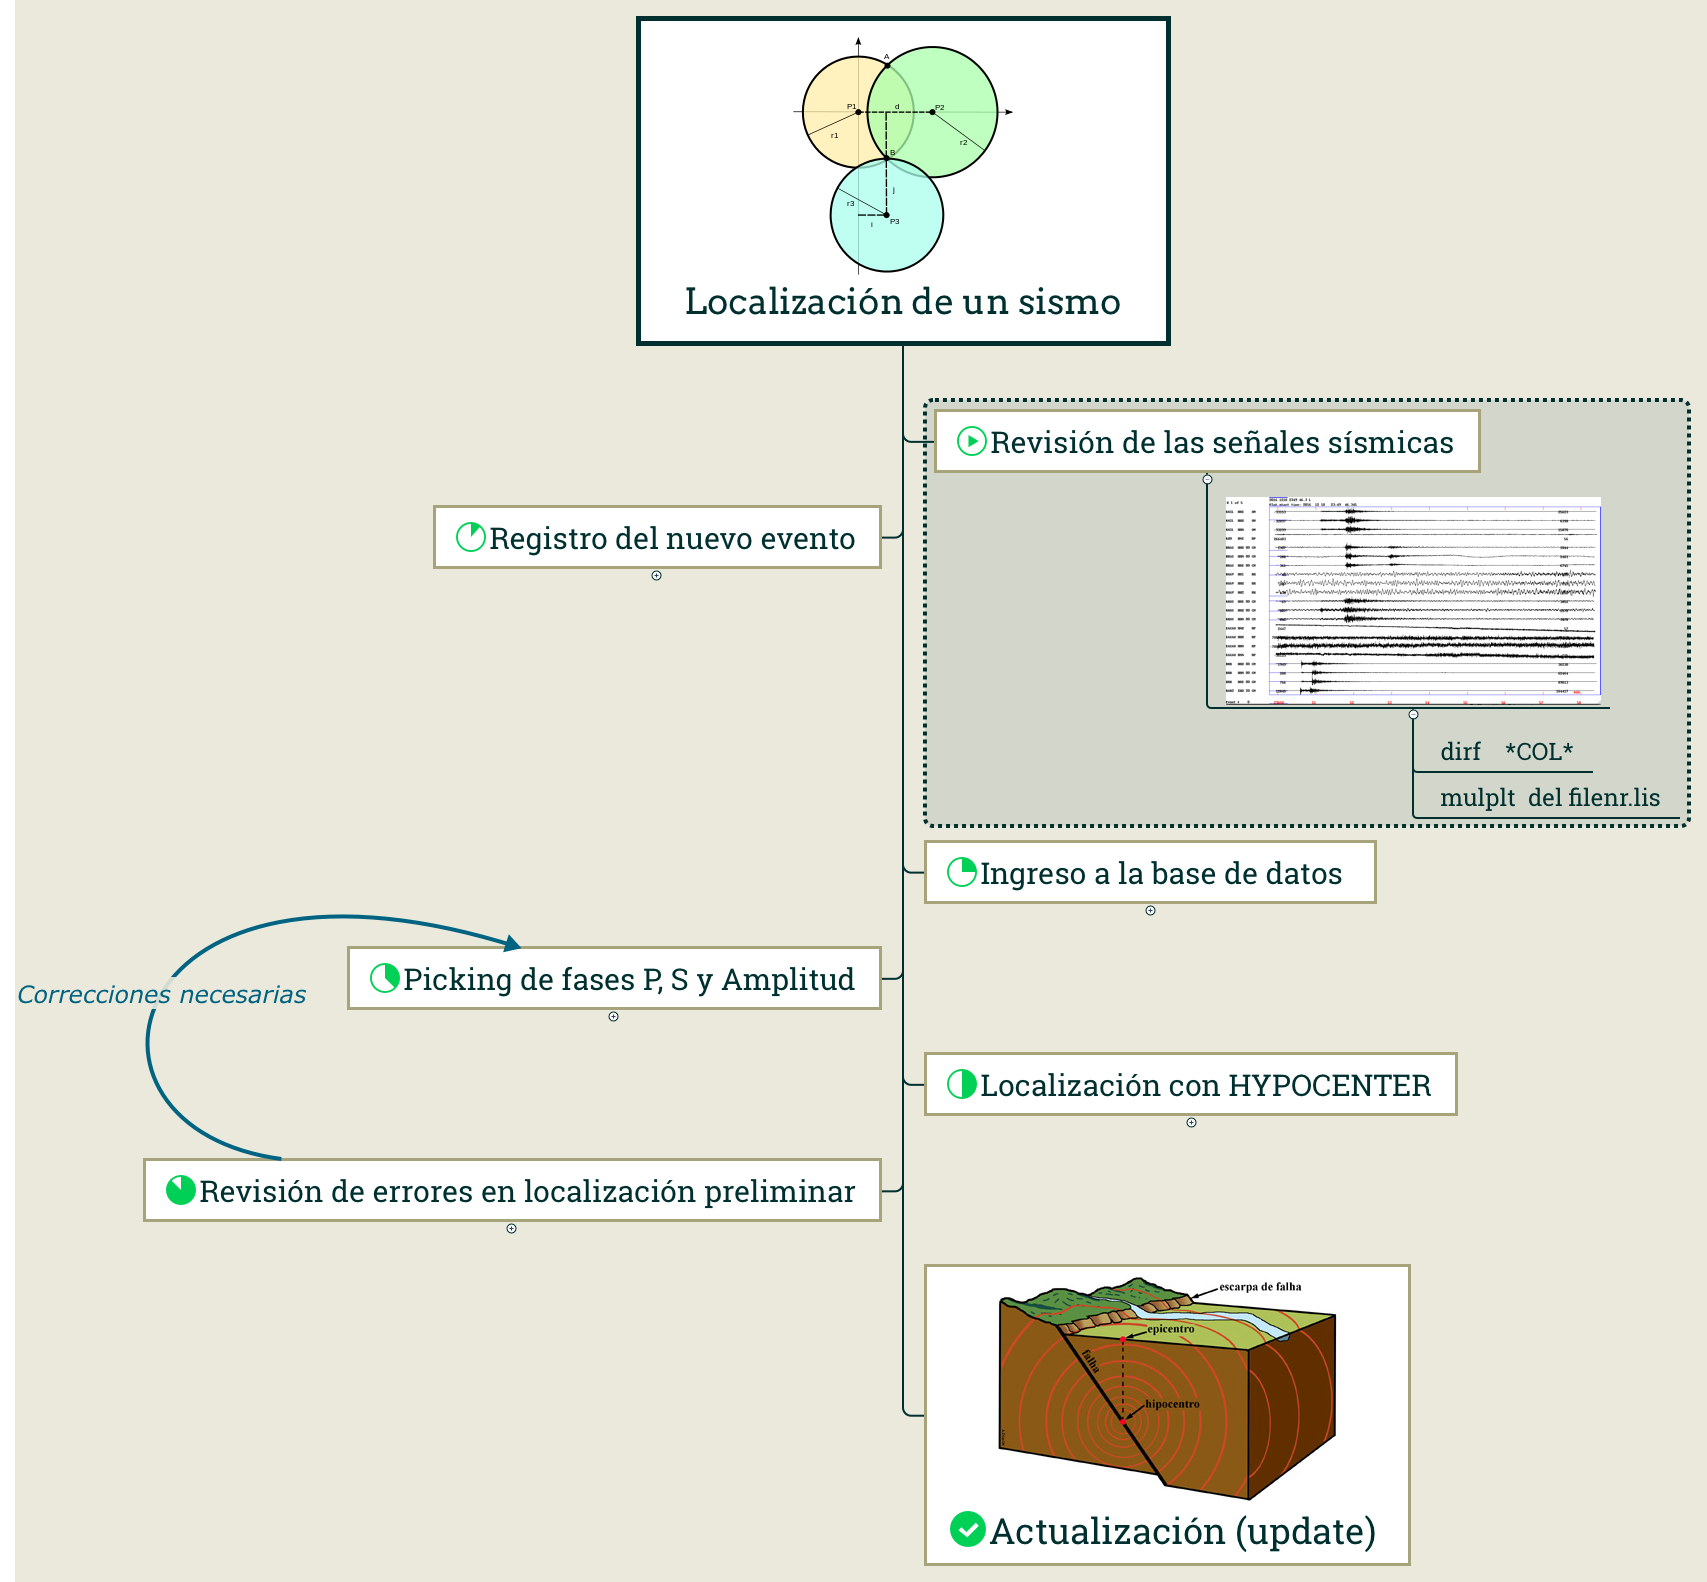
\includegraphics[scale=0.15]{localizacion_2.png}
\end{figure}
\end{frame}

\begin{frame}{Localización en SEISAN}
\begin{figure}
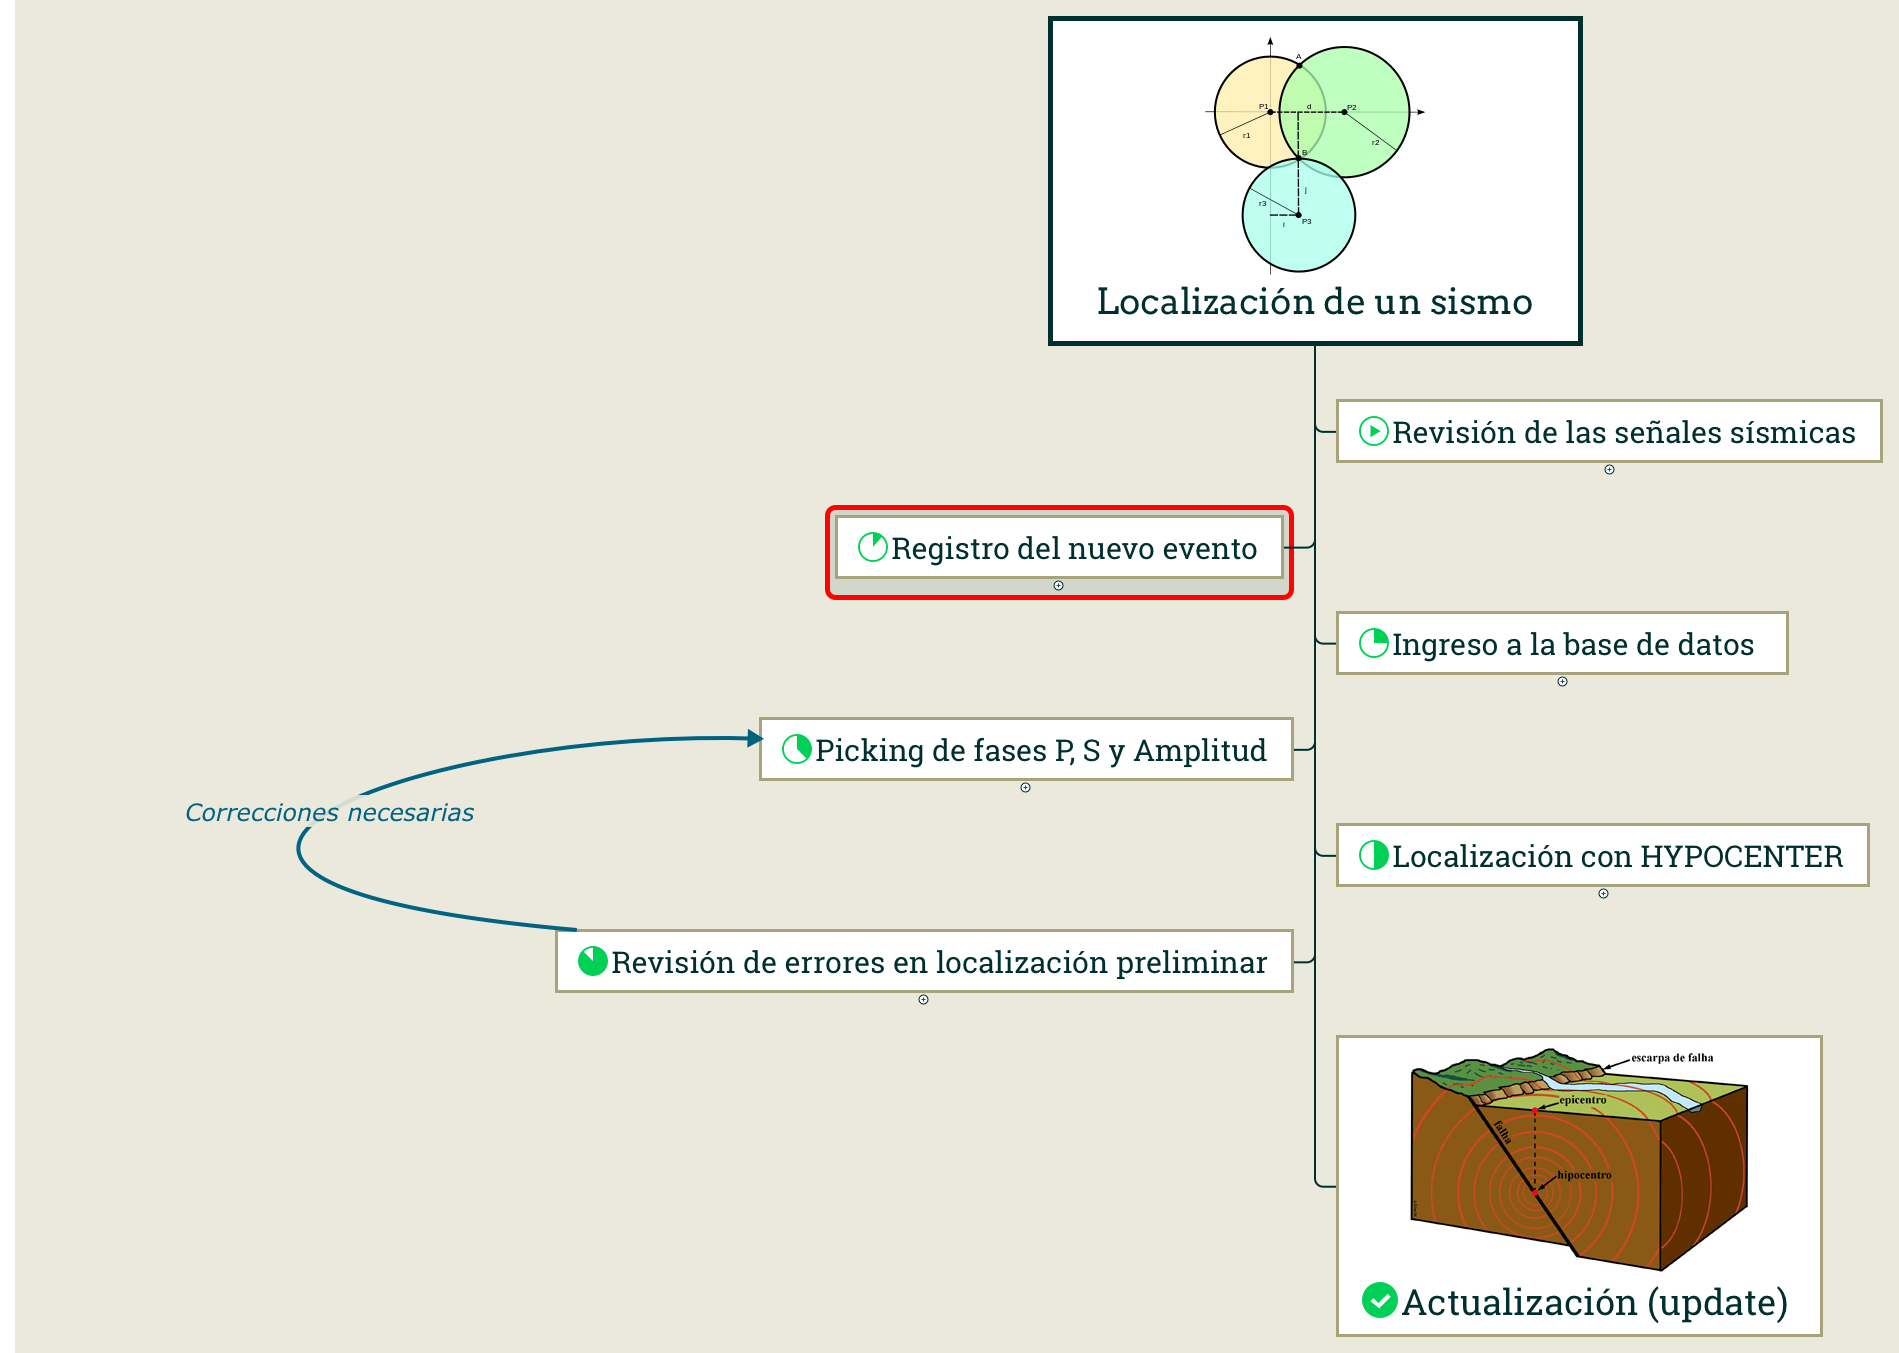
\includegraphics[scale=0.15]{localizacion_1_2.png}
\end{figure}
\end{frame}

\begin{frame}{Localización en SEISAN}
\begin{figure}
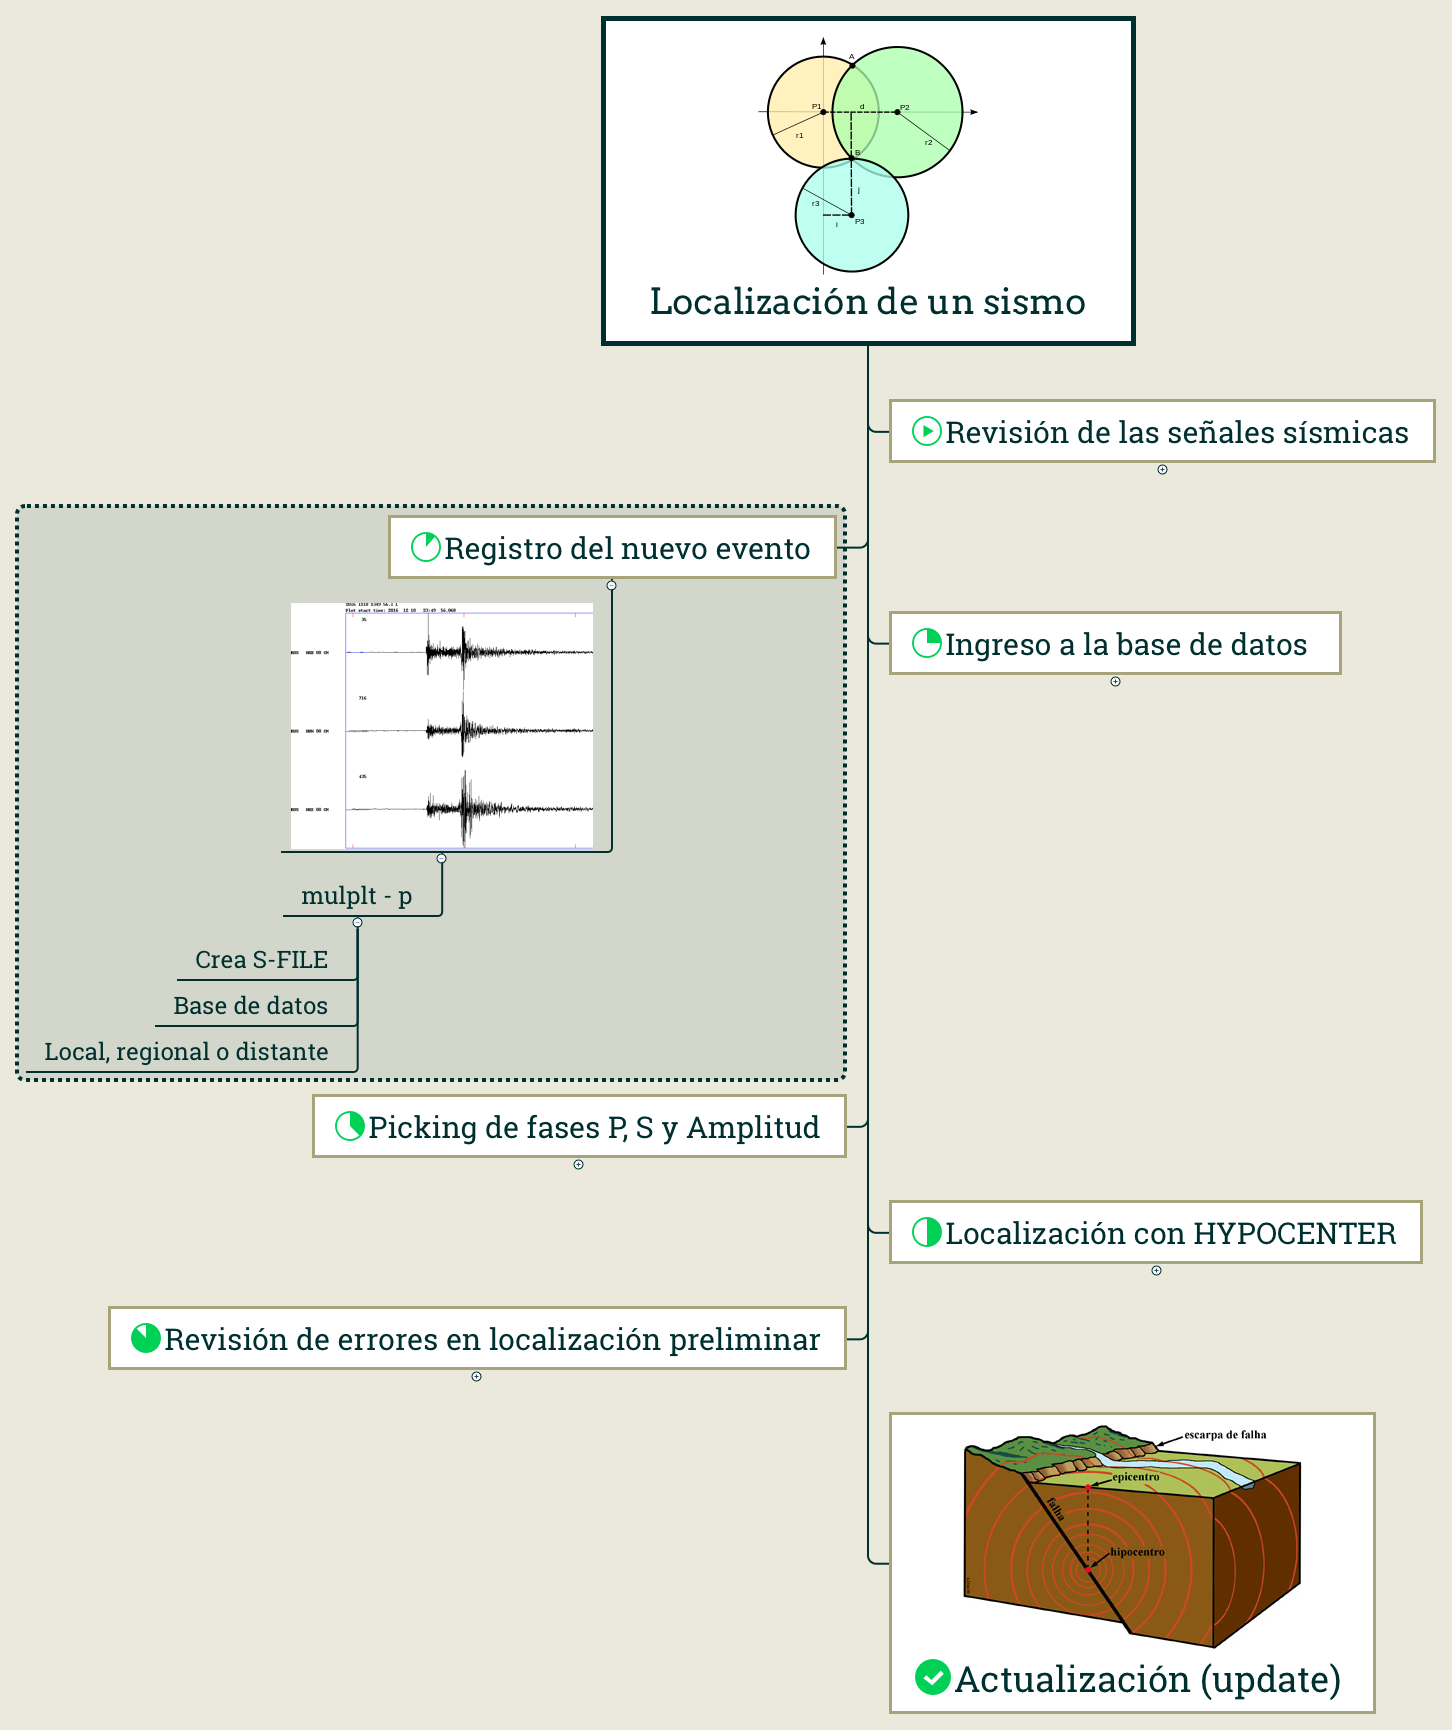
\includegraphics[scale=0.15]{localizacion_3.png}
\end{figure}
\end{frame}

\begin{frame}{Localización en SEISAN}
\begin{figure}
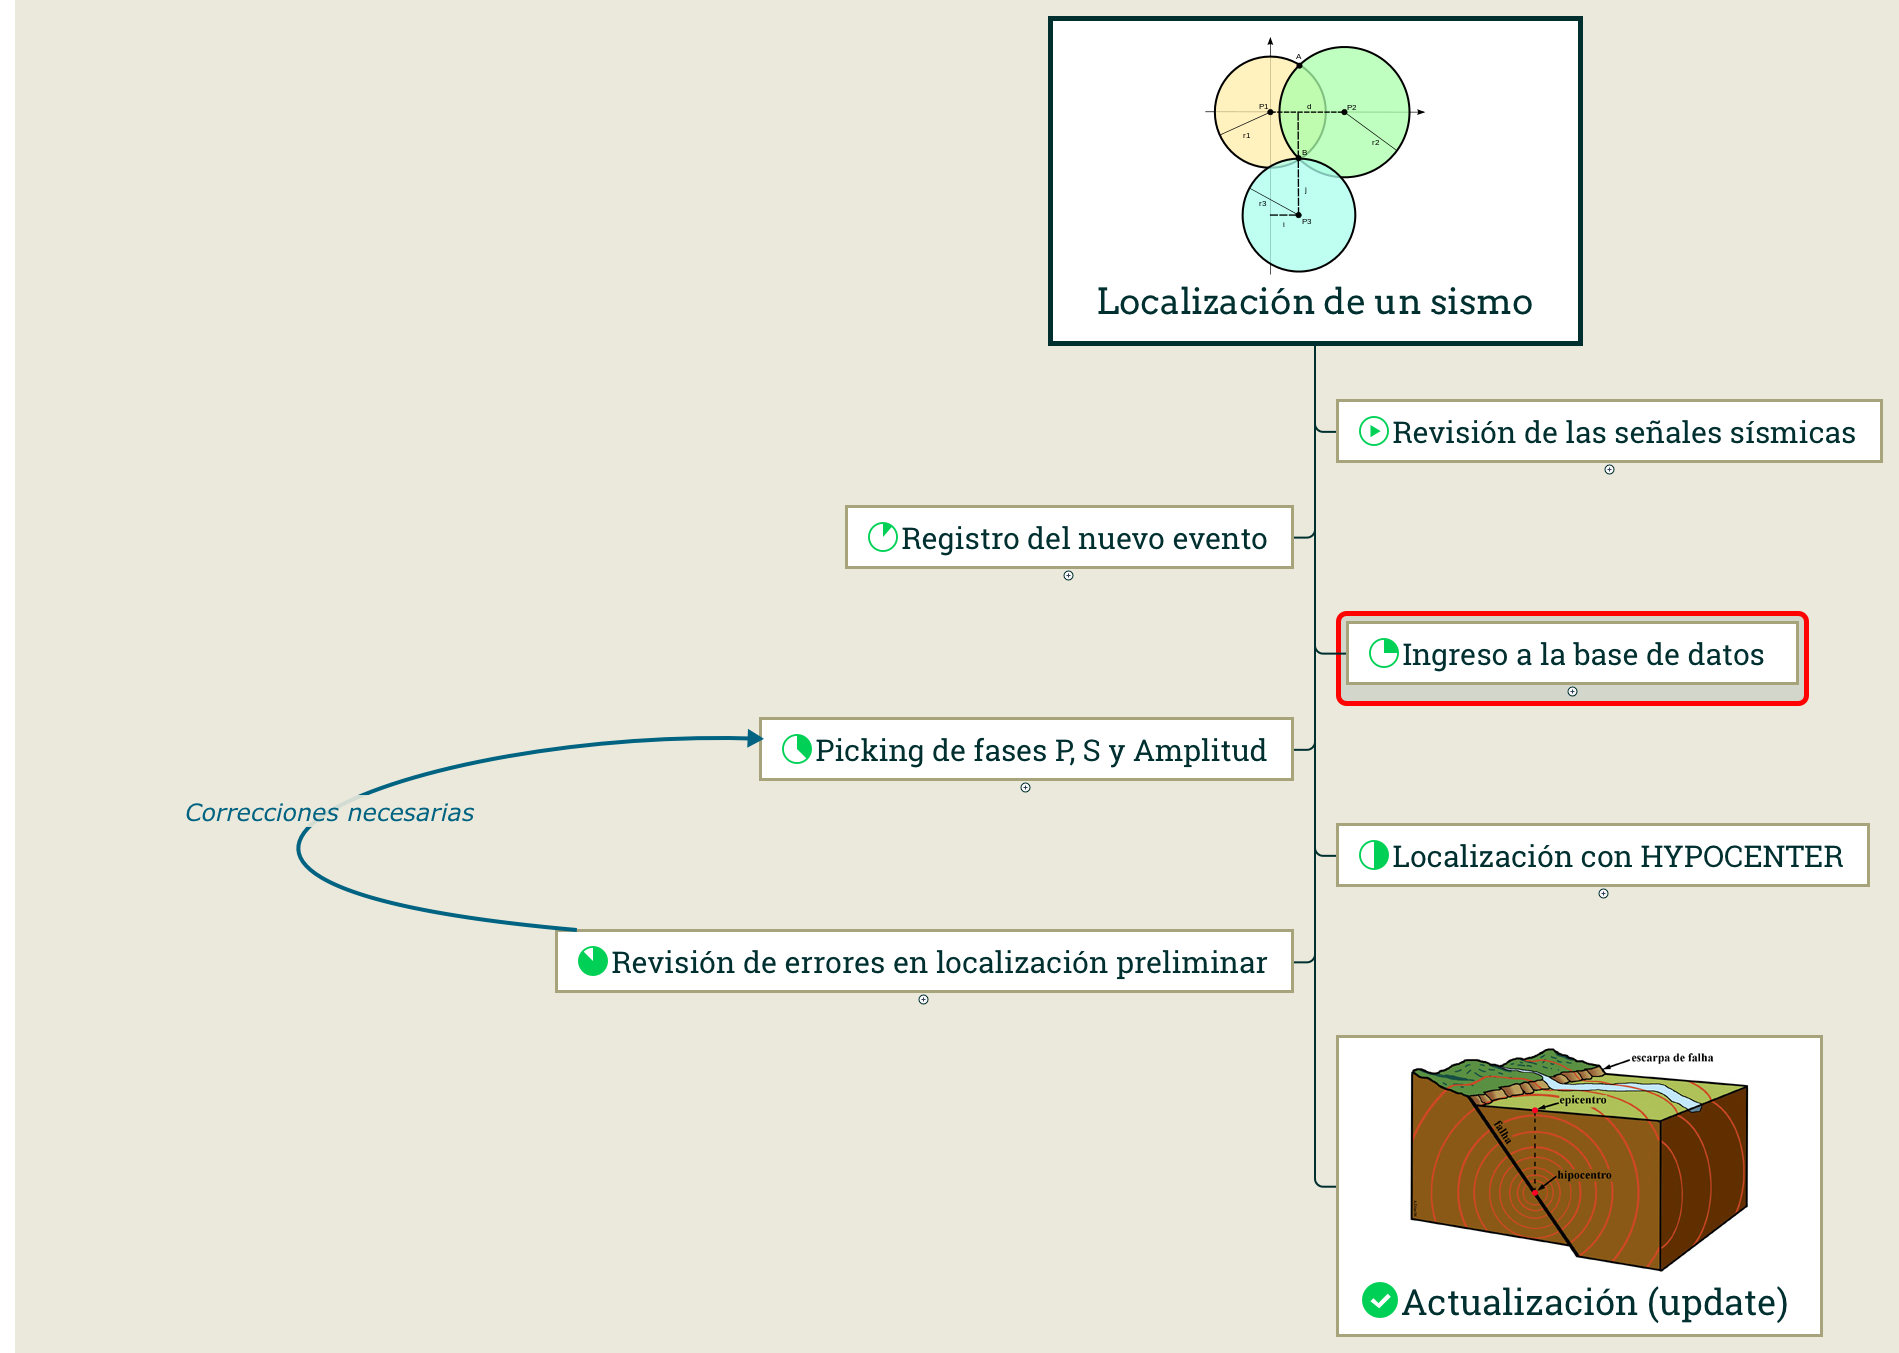
\includegraphics[scale=0.15]{localizacion_1_3.png}
\end{figure}
\end{frame}

\begin{frame}{Localización en SEISAN}
\begin{figure}
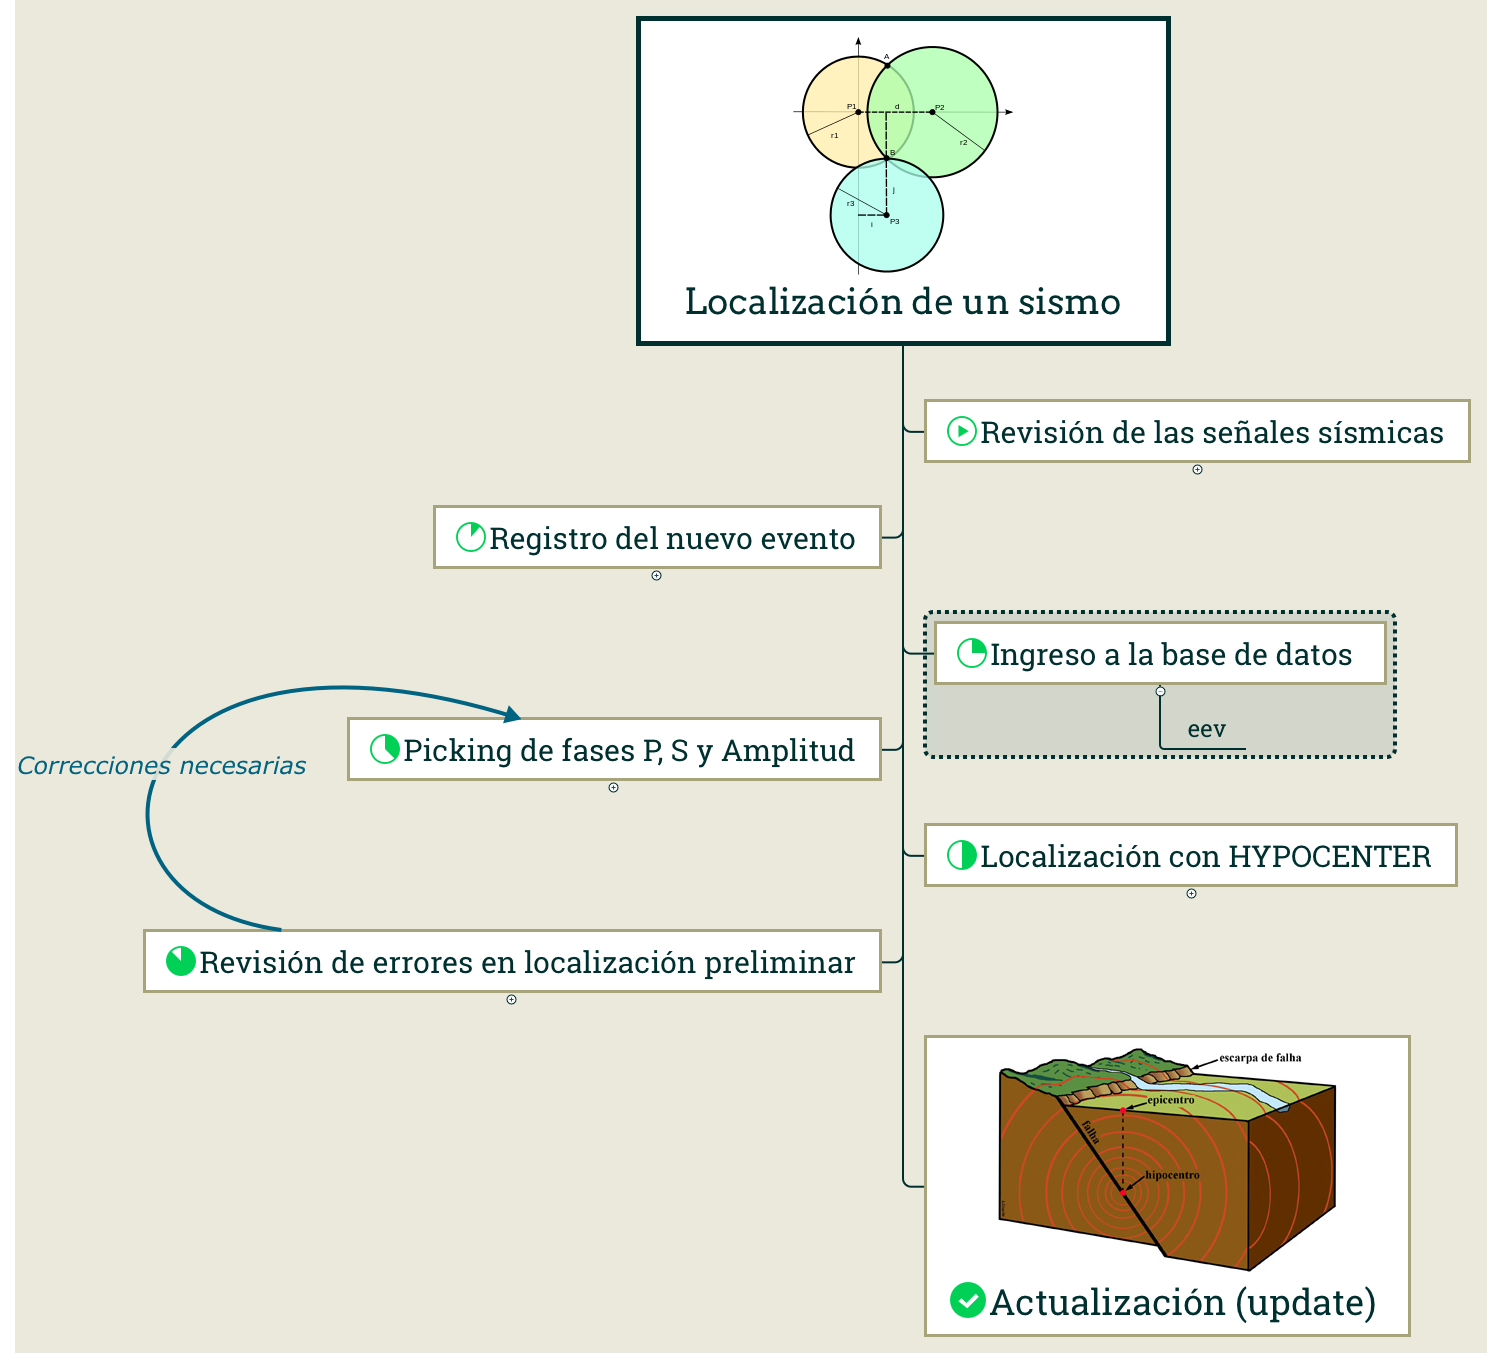
\includegraphics[scale=0.15]{localizacion_4.png}
\end{figure}
\end{frame}

\begin{frame}{Localización en SEISAN}
\begin{figure}
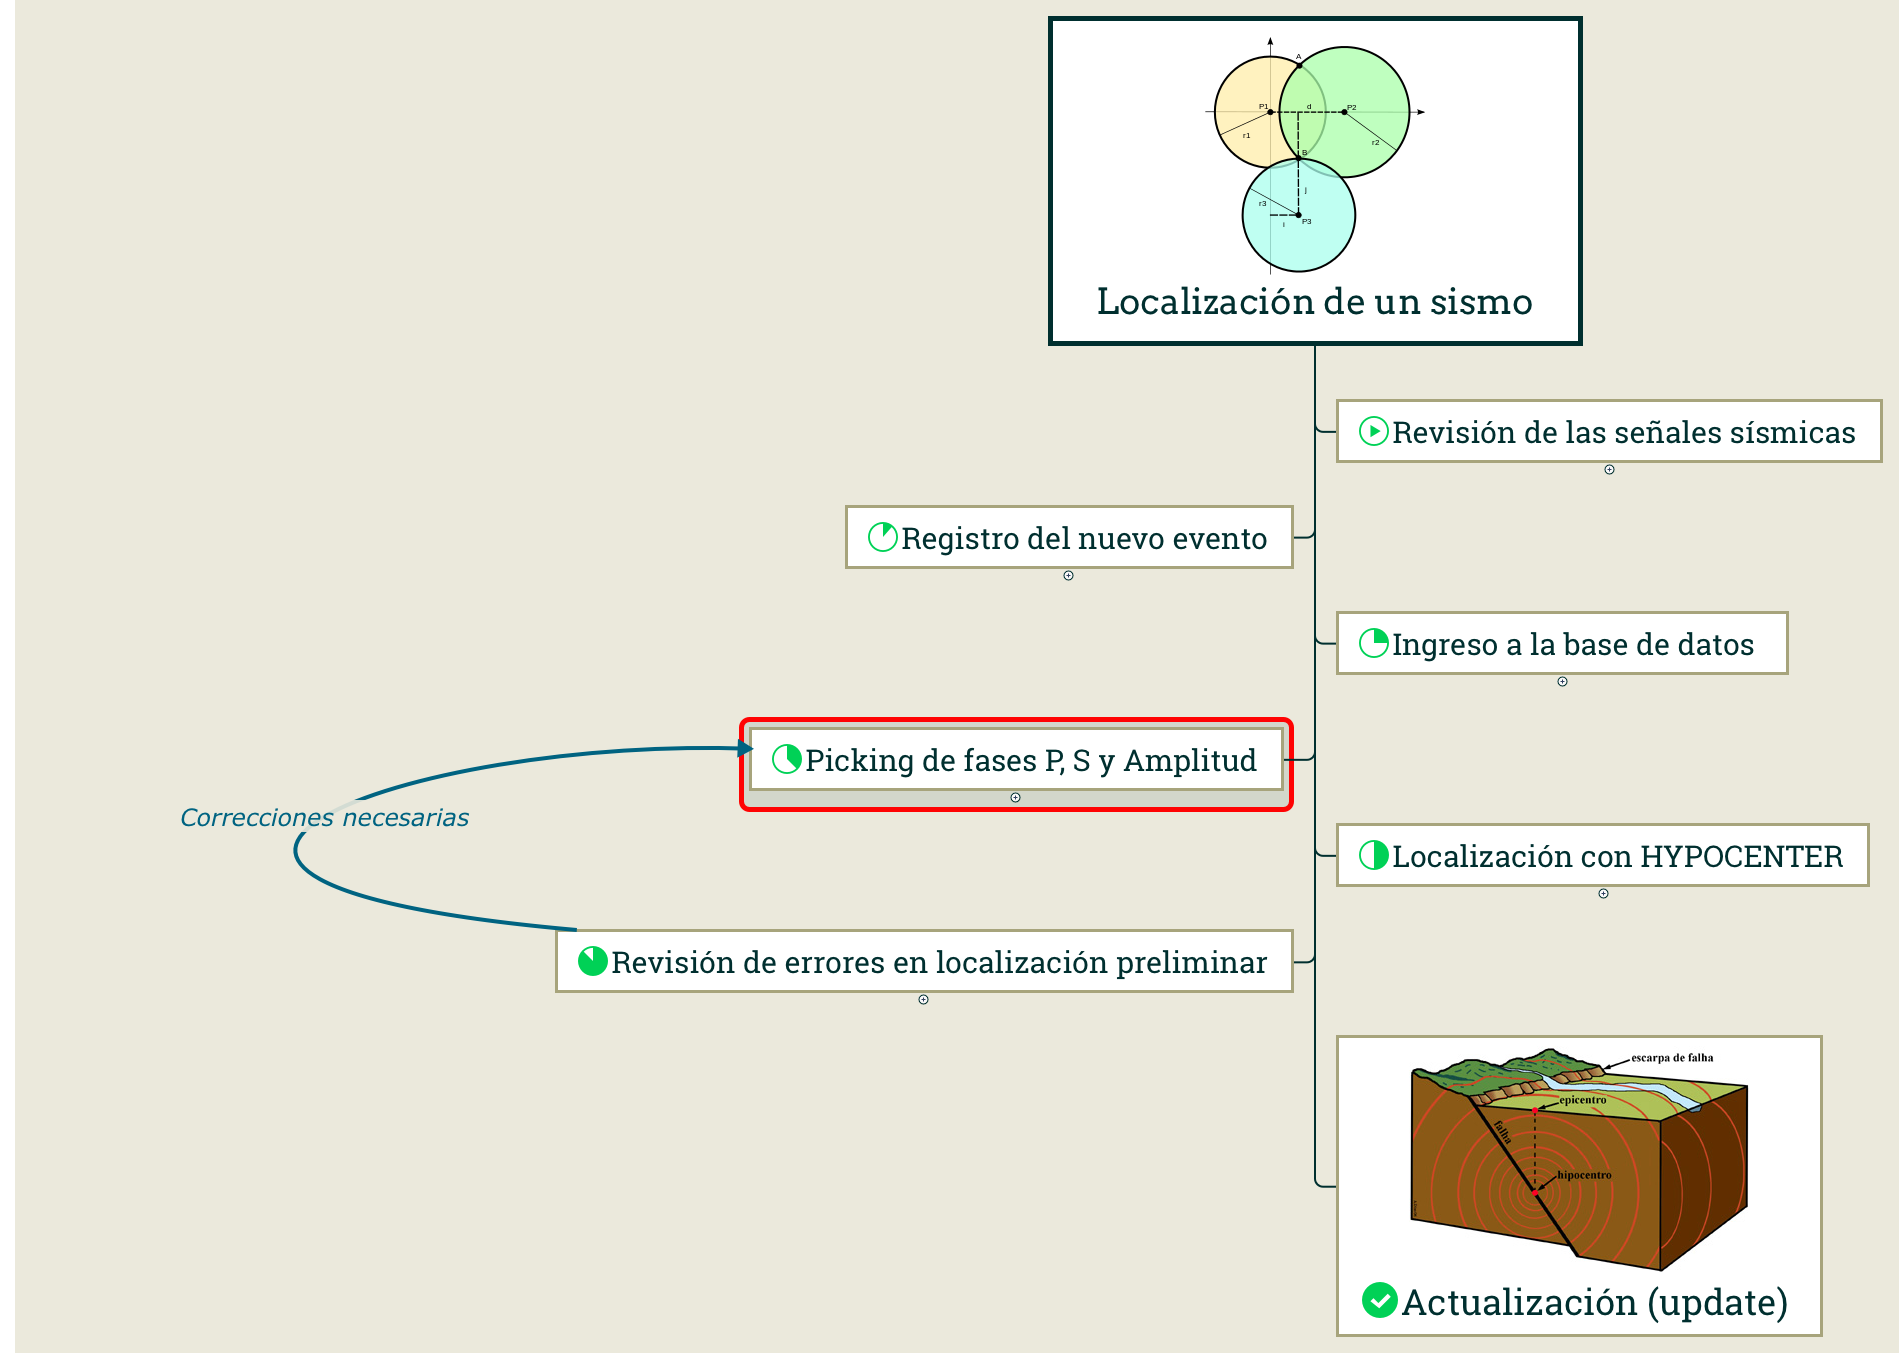
\includegraphics[scale=0.15]{localizacion_1_4.png}
\end{figure}
\end{frame}

\begin{frame}{Localización en SEISAN}
\begin{figure}
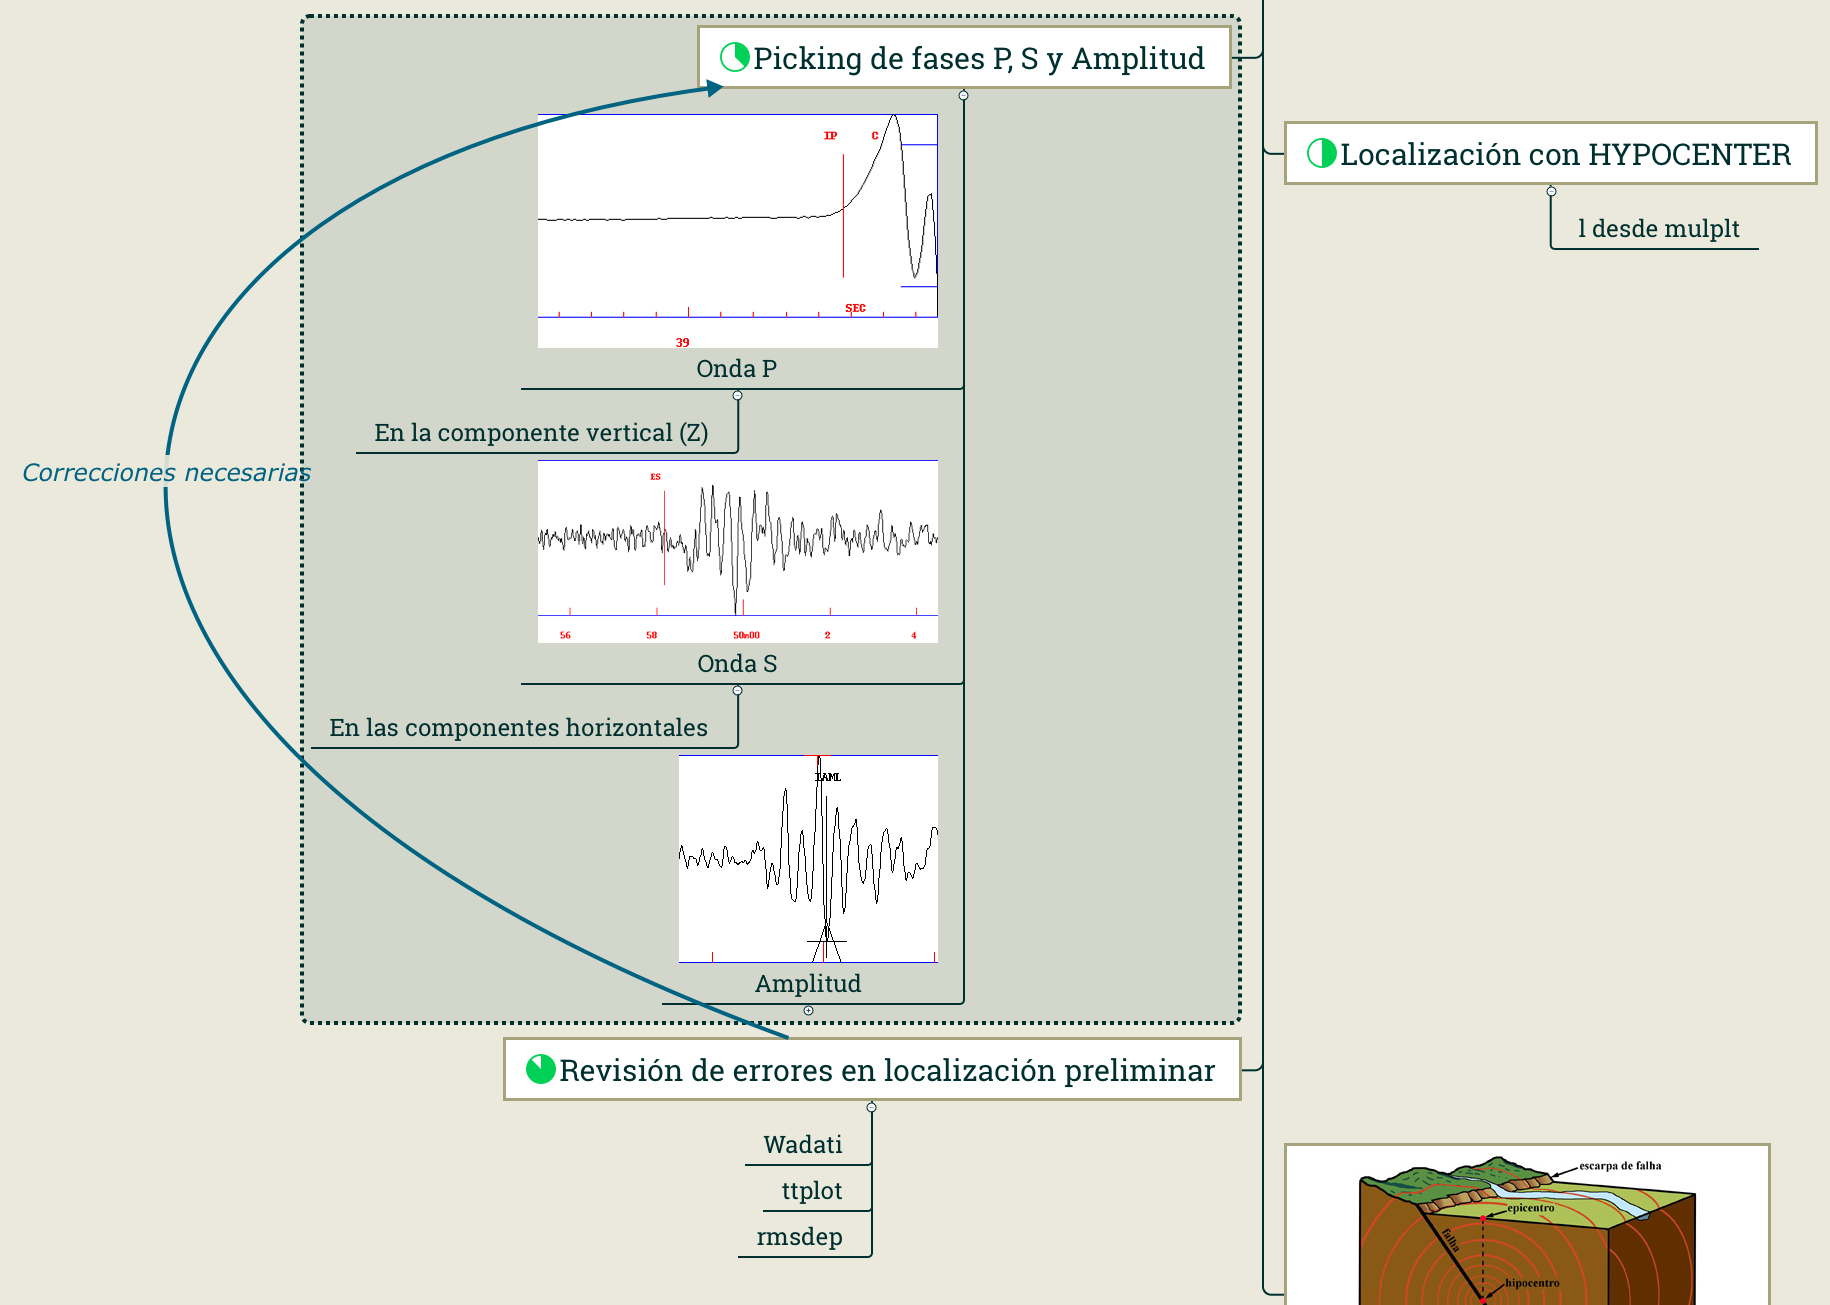
\includegraphics[scale=0.15]{localizacion_5.png}
\end{figure}
\end{frame}

\begin{frame}{Localización en SEISAN}
\begin{figure}
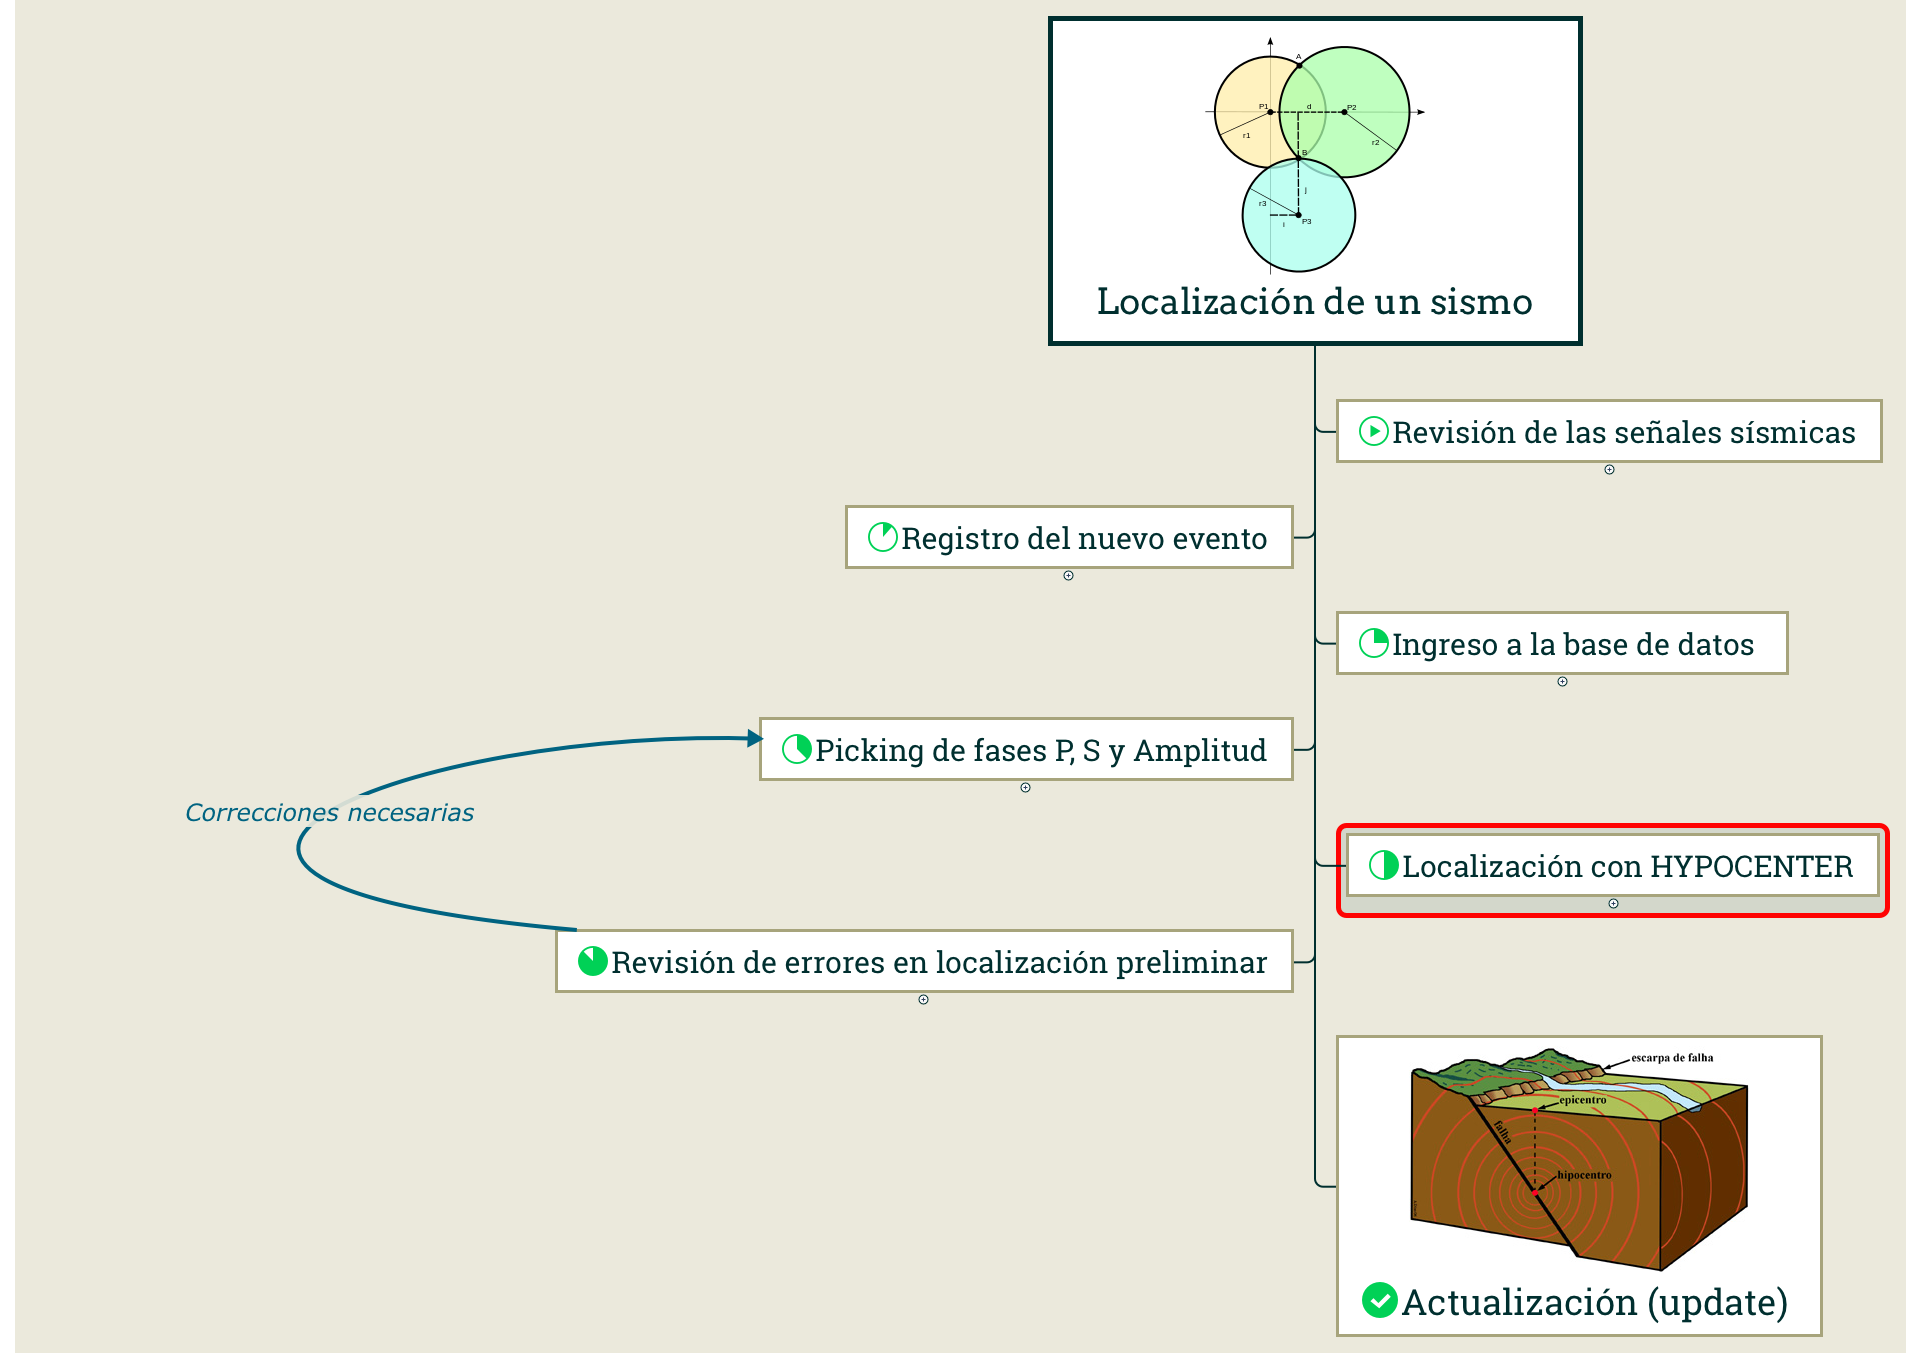
\includegraphics[scale=0.15]{localizacion_1_5.png}
\end{figure}
\end{frame}

\begin{frame}{Localización en SEISAN}
\begin{figure}
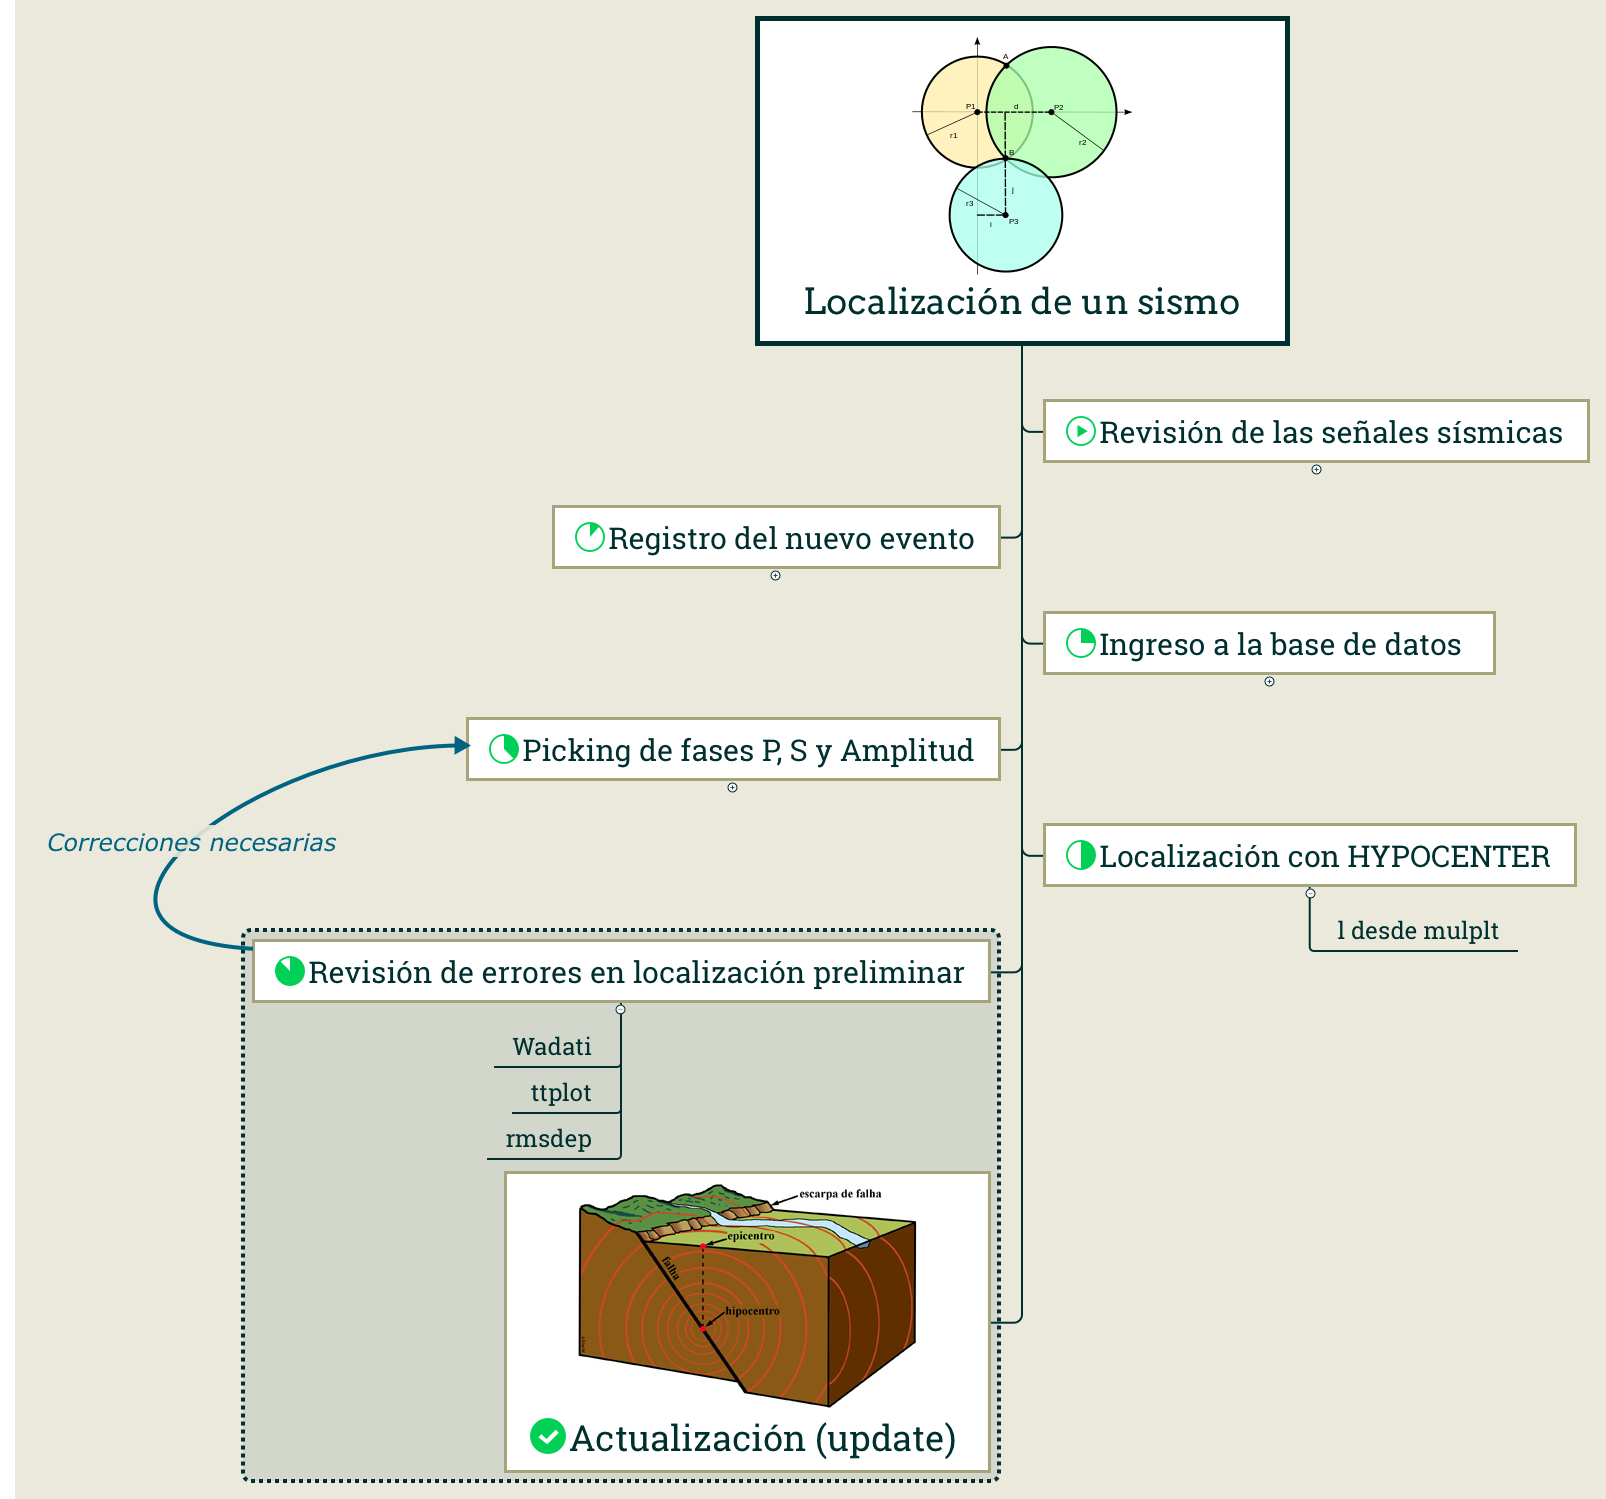
\includegraphics[scale=0.13]{localizacion_6.png}
\end{figure}
\end{frame}

\end{document}